\reportchapter{4}{R\'{e}alisation et Impl\'{e}mentation}{Environnement de d\'{e}veloppement, pipeline d'ingestion \`{a} trois niveaux, classifier \`{a} deux couches, extracteurs m\'{e}tier d\'{e}di\'{e}s, validation Modulo~97, cross-r\'{e}f\'{e}rence crois\'{e}e, backend FastAPI, frontend SPA et blocs de code source comment\'{e}s.}

\section*{Introduction}

Ce chapitre d\'{e}taille la r\'{e}alisation technique du syst\`{e}me de v\'{e}rification documentaire. Il pr\'{e}sente l'environnement de d\'{e}veloppement, le pipeline d'ingestion \`{a} trois niveaux, le classifier \`{a} deux couches, les sept extracteurs m\'{e}tier d\'{e}di\'{e}s, les validateurs math\'{e}matiques (Modulo~97), le moteur de cross-r\'{e}f\'{e}rence, le backend FastAPI, le frontend SPA et les principaux blocs de code source. Chaque composant est illustr\'{e} par des listings comment\'{e}s extraits directement du code source du projet.

\section{Environnement de D\'{e}veloppement}

\begin{table}[H]
\centering
\small
\begin{tabularx}{\textwidth}{@{}>{\bfseries}p{3.5cm} Y@{}}
\toprule
\rowcolor{lightblue}
\'{E}l\'{e}ment & Configuration \\
\midrule
Syst\`{e}me d'exploitation & Windows 11 / macOS \\
Langage & Python 3.11 \\
IDE & Visual Studio Code avec extensions Python, LaTeX \\
Gestion de version & Git / GitHub \\
Base de donn\'{e}es & PostgreSQL 15 (conteneur Docker) \\
Serveur web & uvicorn (ASGI) \\
Tests & pytest 7.x \\
\bottomrule
\end{tabularx}
\caption{Environnement de d\'{e}veloppement du projet.}
\label{tab:environnement-dev}
\end{table}

Les d\'{e}pendances Python du projet sont g\'{e}r\'{e}es via le fichier \texttt{requirements.txt} :

\begin{lstlisting}[language=Python, caption={D\'{e}pendances principales du projet.}, label={lst:requirements}]
rapidfuzz>=3.0.0        # Correspondance floue
pymupdf>=1.22.0         # Extraction PDF
pydantic>=2.0.0         # Modeles de donnees
python-dateutil>=2.8.2  # Manipulation de dates
pytest>=7.0.0           # Tests unitaires
fastapi>=0.100.0        # Framework API
psycopg2-binary>=2.9.0  # Driver PostgreSQL
uvicorn>=0.23.0         # Serveur ASGI
\end{lstlisting}

\subsection{Challenge d'Ing\'{e}nierie de Donn\'{e}es : Constitution du Jeu de Test Coh\'{e}rent et \'{E}dition Canva}

L'un des d\'{e}fis d'ing\'{e}nierie majeurs rencontr\'{e}s lors du d\'{e}veloppement a \'{e}t\'{e} la constitution d'un **jeu de donn\'{e}es de test multi-documents r\'{e}aliste et parfaitement coh\'{e}rent**.

\begin{figure}[H]
    \centering
    \IfFileExists{Logos/Logo_Canva.png}{
\includegraphics[height=1.4cm]{Logos/Logo_Canva.png}}{\fbox{\textbf{Canva PDF Editor}}}
    \caption{Outil d'\'{e}dition vectorielle PDF Canva utilis\'{e} pour la constitution du jeu de données.}
    \label{fig:logo-canva}
\end{figure}

\begin{riskbox}
\textbf{Probl\'{e}matique de D\'{e}part : Incoh\'{e}rence des Échantillons Web (Scribd)} \\
Pour des raisons de confidentialit\'{e} et de conformit\'{e} CNDP/RGPD, les documents administratifs d'entreprises marocaines r\'{e}elles ne sont pas accessibles en open data. Les sp\'{e}cimens isol\'{e}s r\'{e}cup\'{e}r\'{e}s sur des plateformes publiques (ex: Scribd) appartenaient \`{a} des entreprises totalement distinctes. Leurs identifiants (ICE, IF, RC, Raison Sociale, RIB, G\'{e}rant) ne concordaient aucunement d'un document \`{a} l'autre, rendant impossible la recette de la Matrice de Coh\'{e}rence Crois\'{e}e (\textit{Cross-Reference Matrix}).
\end{riskbox}

\subsubsection{M\'{e}thodologie de R\'{e}solution et Point d'Ancrage Scann\'{e}}

Pour simuler un dossier de souscription r\'{e}el et valide soumis par un op\'{e}rateur \'{e}conomique, une d\'{e}marche d'harmonisation a \'{e}t\'{e} mise en \oe{}uvre :

\begin{enumerate}[leftmargin=*, itemsep=4pt]
    \item \textbf{Identification des Contraintes d'Inalt\'{e}rabilit\'{e} (Documents Scann\'{e}s)} : La Carte Nationale d'Identit\'{e} (\textbf{CNIE}) et l'\textbf{Attestation RIB} (Bank of Africa) sont des documents scann\'{e}s sous forme d'images matricielles (pixels). Contrairement aux PDF vectoriels, ils ne peuvent pas \^{e}tre \'{e}dit\'{e}s textuellement sans alt\'{e}ration visuelle ou falsification perceptible.
    \item \textbf{Choix des Points d'Ancrage Immuables} : L'ing\'{e}nieur a utilis\'{e} une CNIE sp\'{e}cimen (\texttt{AB123456}, g\'{e}rant \textsc{BOUALAM MOHAMED}) et un RIB bancaire officiel (\texttt{011780000009210006415609}) comme **pivots d'ancrage absolus**.
    \item \textbf{Harmonisation Vectorielle via Canva} : Tous les autres documents du dossier vectoriels (Mod\`{e}le J, Bulletin IF, Certificat ICE, Taxe Professionnelle, Domiciliation, Statuts) ont \'{e}t\'{e} import\'{e}s dans l'outil d'\'{e}dition PDF **Canva** (voir figure~\ref{fig:logo-canva}). Les champs texte vectoriels ont \'{e}t\'{e} modifi\'{e}s pour faire r\'{e}f\'{e}rence \`{a} l'entit\'{e} centrale \texttt{MEDI TELECOM S.A.} / \texttt{GOAL VOYAGES}, au g\'{e}rant \textsc{BOUALAM MOHAMED} et \`{a} l'ICE \texttt{001512572000078}.
\end{enumerate}

Cette ing\'{e}nierie de donn\'{e}es a permis de disposer d'un jeu de test de 9 pi\`{e}ces parfaitement interconnect\'{e}es, validant l'int\'{e}gralit\'{e} des r\`{e}gles de cross-r\'{e}f\'{e}rence du syst\`{e}me.

\section{Pipeline d'Ingestion \`{a} Trois Niveaux}

Le pipeline de traitement est orchestr\'{e} par la classe \texttt{Orchestrator}, qui coordonne trois niveaux de traitement s\'{e}quentiels illustr\'{e}s dans la figure~\ref{fig:pipeline-ingestion} :

\begin{figure}[H]
    \centering
    \IfFileExists{images/pipeline_ingestion.png}{\includegraphics[width=\textwidth]{images/pipeline_ingestion.png}}{\fbox{\parbox{14cm}{\centering\vspace{2.5cm}\textit{Pipeline d'ingestion \`{a} trois niveaux --- Exporter depuis pipeline\_ingestion.drawio}\vspace{2.5cm}}}}
    \caption{Pipeline d'ingestion et de traitement \`{a} trois niveaux.}
    \label{fig:pipeline-ingestion}
\end{figure}

\subsection{Niveau 1 : Extraction Textuelle}

Le premier niveau extrait le texte brut du fichier PDF. La strat\'{e}gie d'extraction combine deux m\'{e}thodes :

\begin{lstlisting}[language=Python, caption={Extraction PDF avec repli OCR (orchestrator.py).}, label={lst:extraction}]
# Phase 1: Extraction du texte vectoriel natif
raw_text = extract_pdf_text(path)
is_scanned = len(raw_text.strip()) < 20

# Phase 2: Repli OCR si le document est numerise
if is_scanned:
    raw_text = run_ocr(path)
\end{lstlisting}

La fonction \texttt{extract\_pdf\_text} utilise PyMuPDF pour acc\'{e}der directement aux op\'{e}rateurs de texte du PDF, avec un temps d'extraction typique inf\'{e}rieur \`{a} 100~ms par page. Le seuil de 20 caract\`{e}res permet de d\'{e}tecter les documents purement rasteris\'{e}s (scans) qui n\'{e}cessitent le recours \`{a} l'OCR.

\subsection{Niveau 2 : Classification par Emplacement}

Le deuxi\`{e}me niveau v\'{e}rifie que le document d\'{e}pos\'{e} correspond bien \`{a} l'emplacement choisi par l'op\'{e}rateur. Le classifier \`{a} deux couches constitue l'innovation algorithmique principale du projet :

\begin{figure}[H]
    \centering
    \IfFileExists{images/classifier_2_couches.png}{
\includegraphics[width=\textwidth]{images/classifier_2_couches.png}}{\fbox{\parbox{14cm}{\centering\vspace{2cm}\textit{Classifier \`{a} deux couches --- Exporter depuis classifier\_2\_couches.drawio}\vspace{2cm}}}}
    \caption{Fonctionnement du classifier \`{a} deux couches (ancres positives + exclusions n\'{e}gatives).}
    \label{fig:classifier-2-couches}
\end{figure}

\begin{lstlisting}[language=Python, caption={Classifier \`{a} deux couches --- Exemple pour le Mod\`{e}le J (classifier.py).}, label={lst:classifier}]
def verify_slot_document(slot, text):
    """Verification par ancres forensiques."""
    t = text.upper()
    
    # Ancres uniques pour chaque type de document
    _MODEL_J_ANCHORS = ["REGISTRE ANALYTIQUE",
                        "INSCRIPTIONS PORTES",
                        "CODE DEMANDE"]
    _IF_ANCHORS      = ["AAC140B",
                        "BULLETIN DE NOTIFICATION"]
    _TP_ANCHORS      = ["AAC060B"]
    
    if slot == "model_j":
        # Couche 1: Ancres POSITIVES
        has_registry = any(k in t for k in
            ["REGISTRE ANALYTIQUE", "INSCRIPTIONS PORTES"])
        has_code = "CODE DEMANDE" in t
        positive = has_registry or has_code
        
        # Couche 2: Exclusions NEGATIVES
        negative = any(k in t for k in
            _IF_ANCHORS + _TP_ANCHORS)
        
        if positive and not negative:
            return True, DocumentType.MODEL_J, "OK"
        return False, DocumentType.UNKNOWN, "Erreur"
\end{lstlisting}

\begin{riskbox}
\textbf{D\'{e}fi technique : Confusion Domiciliation / Mod\`{e}le~J} \\
L'analyse forensique a r\'{e}v\'{e}l\'{e} que la mention \texttt{ATTESTATION DE DOMICILIATION} appara\^{\i}t \'{e}galement dans le Mod\`{e}le~J comme valeur de champ. Le classifier exige donc un crit\`{e}re suppl\'{e}mentaire : la pr\'{e}sence d'un texte de corps caract\'{e}ristique (\texttt{DONNER DOMICILIATION}, \texttt{SOUSSIGNE}) en conjonction avec le titre.
\end{riskbox}

\subsection{Niveau 3 : Validation et Cross-R\'{e}f\'{e}rence}

Le troisi\'{e}me niveau applique les validations locales (checksums, r\'{e}cence) et la matrice de coh\'{e}rence crois\'{e}e inter-documents.

\section{Extracteurs M\'{e}tier D\'{e}di\'{e}s}

Le syst\`{e}me impl\'{e}mente sept extracteurs sp\'{e}cialis\'{e}s, chacun h\'{e}ritant du mod\`{e}le de base \texttt{ExtractedDocument} et produisant un objet Pydantic structur\'{e} :

\begin{table}[H]
\centering
\small
\begin{tabularx}{\textwidth}{@{}>{\bfseries}p{2.6cm} >{\ttfamily\small\raggedright\arraybackslash}p{3.2cm} Y@{}}
\toprule
\rowcolor{lightblue}
Extracteur & Fichier source & Entit\'{e}s extraites \\
\midrule
Mod\`{e}le J & model\_j.py & D\'{e}nomination, RC, ICE, Forme juridique, Capital, Si\`{e}ge, Date, G\'{e}rants, Activit\'{e} \\
Document IF & document\_if.py & Raison sociale, IF, RC, ICE, TP, Forme juridique, Si\`{e}ge, Date \\
Certificat ICE & ice\_certificate.py & D\'{e}nomination, ICE, IF, RC, Sigle, Date \\
Taxe Prof. & taxe\_pro.py & Raison sociale, IF, ICE, RC, TP, CNI, Si\`{e}ge, Date \\
Attestation RIB & attestation\_rib.py & Raison sociale, RIB (24 chiffres), Code SWIFT, Date \\
Domiciliation & categorie\_op.py & Soci\'{e}t\'{e} domiciliataire, RC domiciliataire, Soci\'{e}t\'{e} domicili\'{e}e, Si\`{e}ge, Dates \\
Statuts & statuts.py & Capital social, Forme juridique, Nom du g\'{e}rant \\
\bottomrule
\end{tabularx}
\caption{Catalogue des sept extracteurs m\'{e}tier et de leurs variables de sortie.}
\label{tab:extracteurs-catalogue}
\end{table}

\begin{lstlisting}[language=Python, caption={Mod\`{e}le de donn\'{e}es Pydantic pour le Mod\`{e}le J (document.py).}, label={lst:model-j-pydantic}]
class ExtractedModelJ(ExtractedDocument):
    document_type: DocumentType = DocumentType.MODEL_J
    denomination: str
    rc_number: str
    rc_city: str
    ice: str
    forme_juridique: str
    capital_social: Optional[float] = None
    siege_social: str
    date_immatriculation: Optional[str] = None
    activite: str
    gerants: List[Gerant] = []
    date_certification: str  # Recency checking
    domiciliary_name: Optional[str] = None
    domiciliary_rc: Optional[str] = None
\end{lstlisting}

\begin{figure}[H]
    \centering
    \IfFileExists{Screenshots/model_j_page1_annotated.png}{
        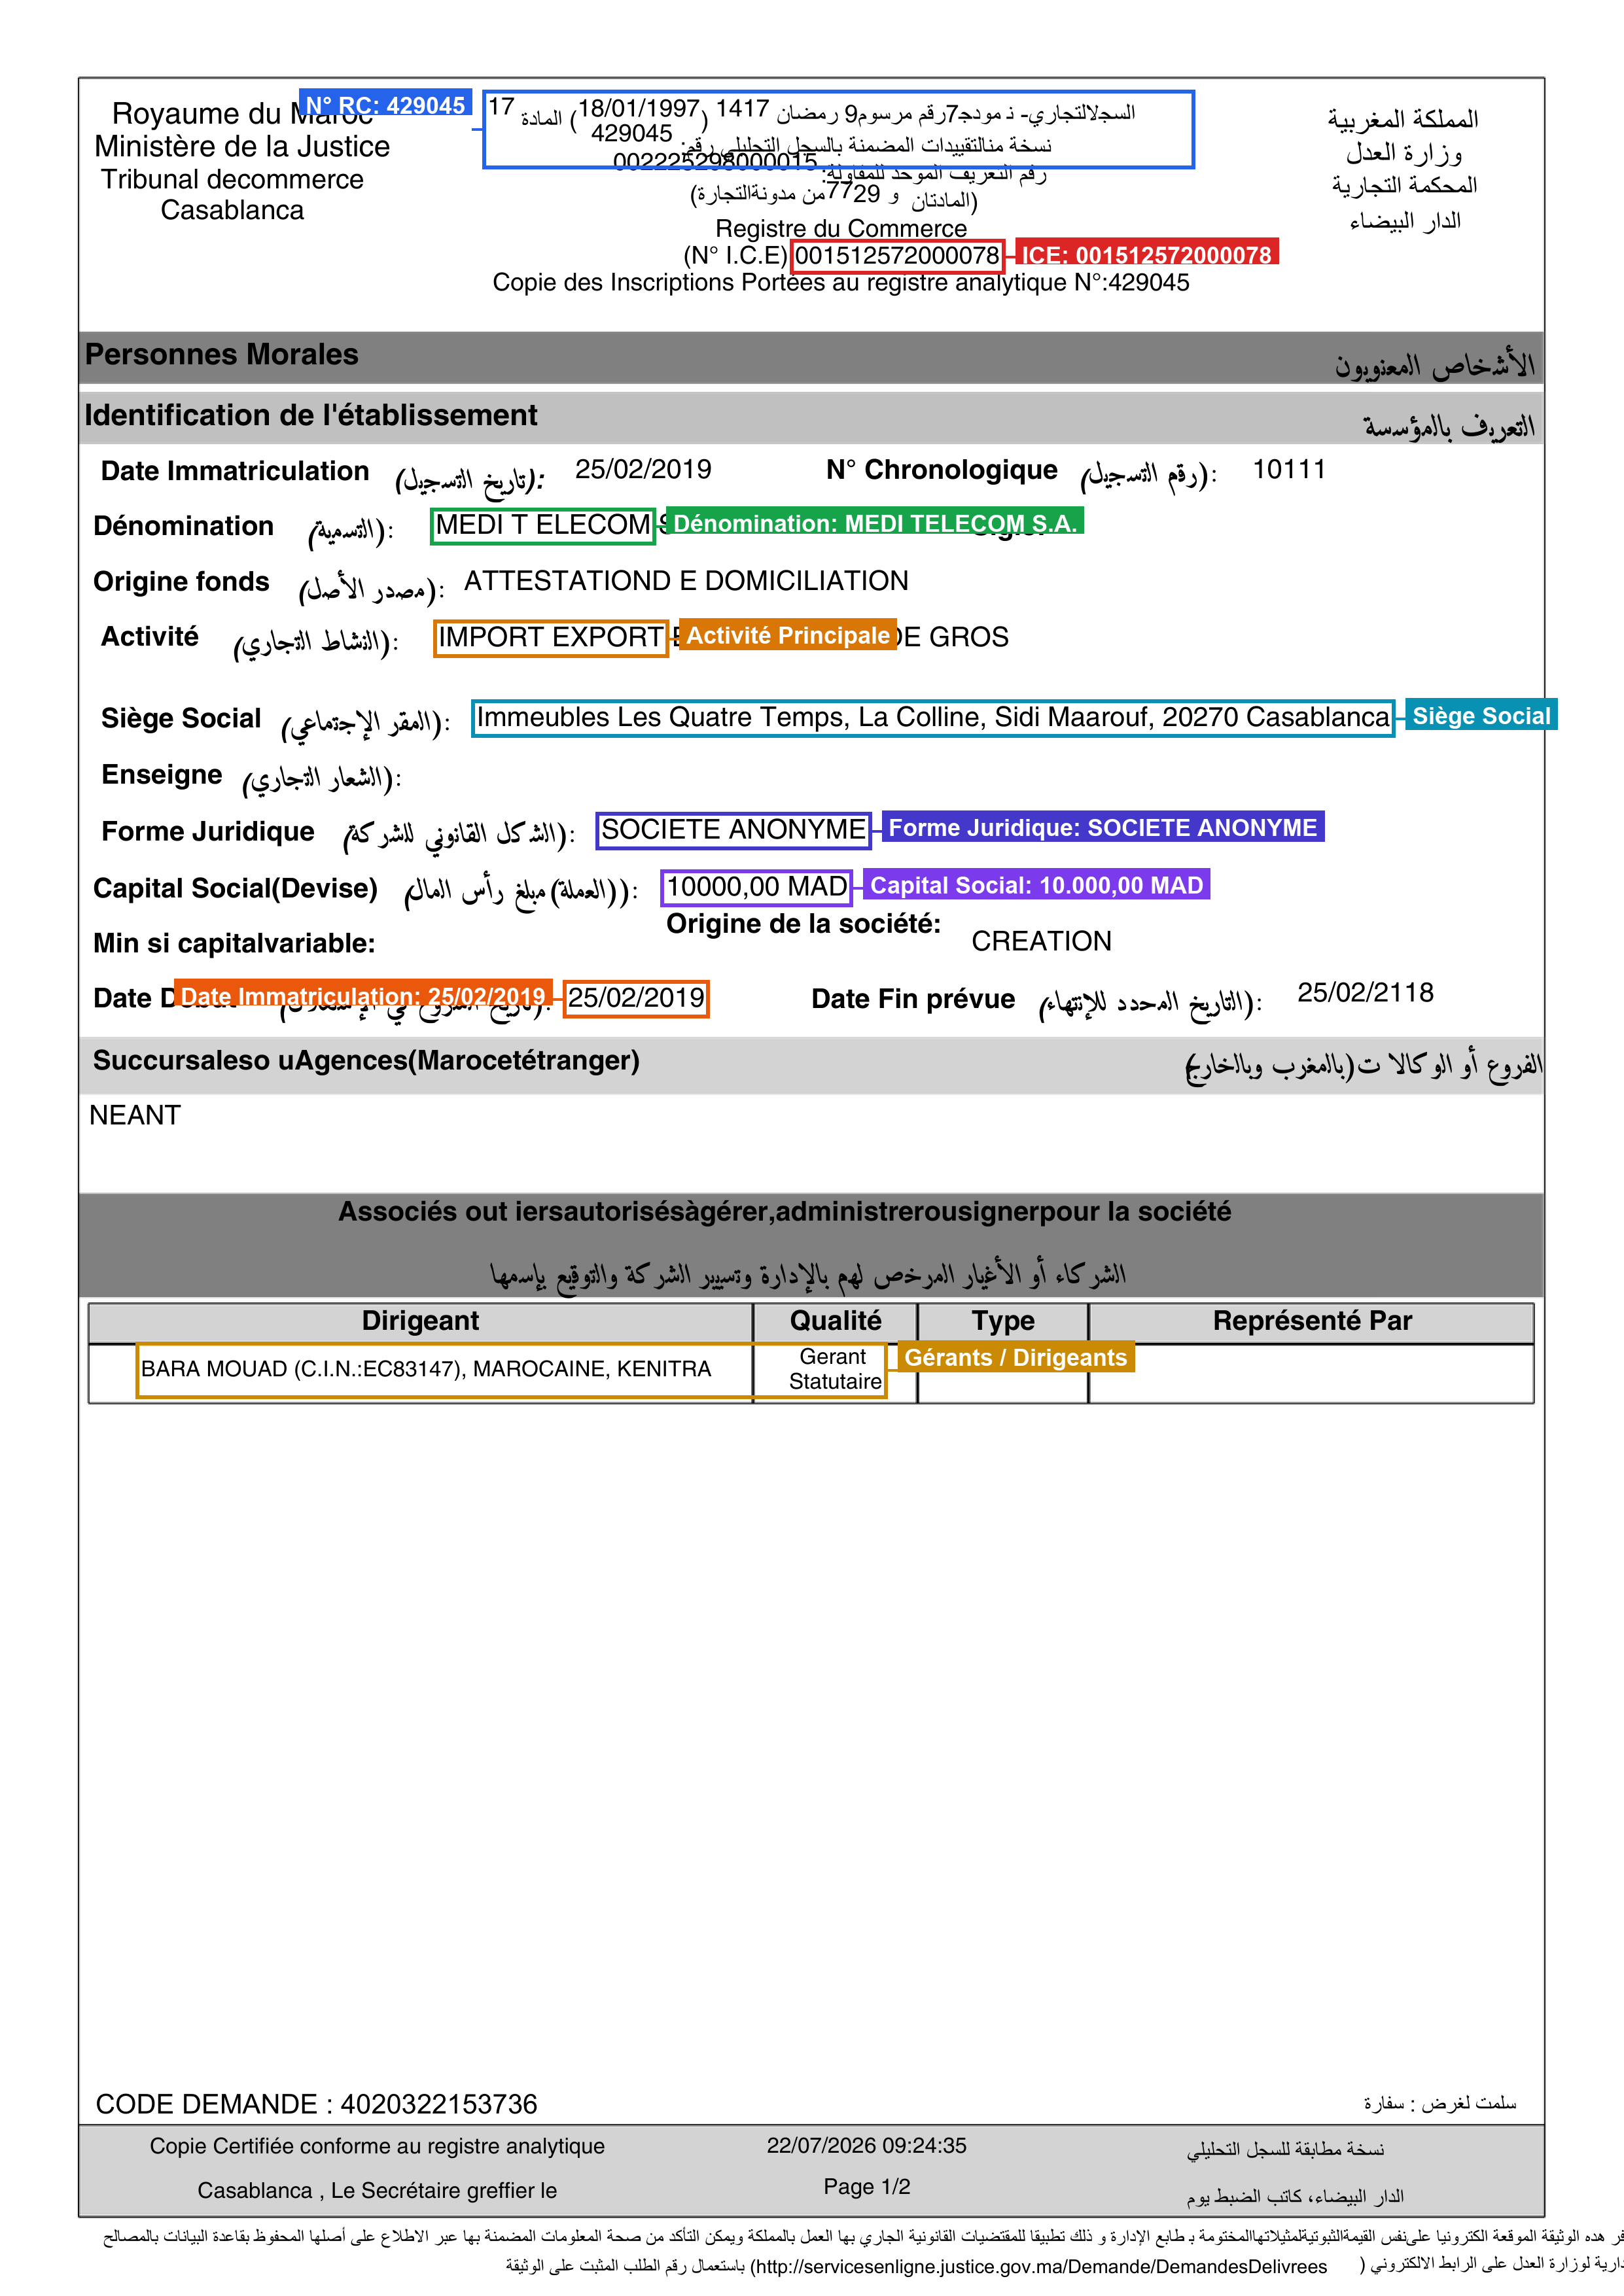
\includegraphics[width=0.72\textwidth]{Screenshots/model_j_page1_annotated.png}
    }{\IfFileExists{Screenshots/model_j_page1_clean.png}{
        \includegraphics[width=0.72\textwidth]{Screenshots/model_j_page1_clean.png}
    }{
        \fbox{\parbox{12cm}{\centering\vspace{2.5cm}\textit{Échantillon Mod\`{e}le J (Page 1)}\vspace{2.5cm}}}
    }}
    \caption{Zones d'extraction sur la Page 1 du Mod\`{e}le J (Fichier valide du jeu de test).}
    \label{fig:model-j-page1-annotated}
\end{figure}

\begin{figure}[H]
    \centering
    \IfFileExists{Screenshots/model_j_page2_annotated.png}{
        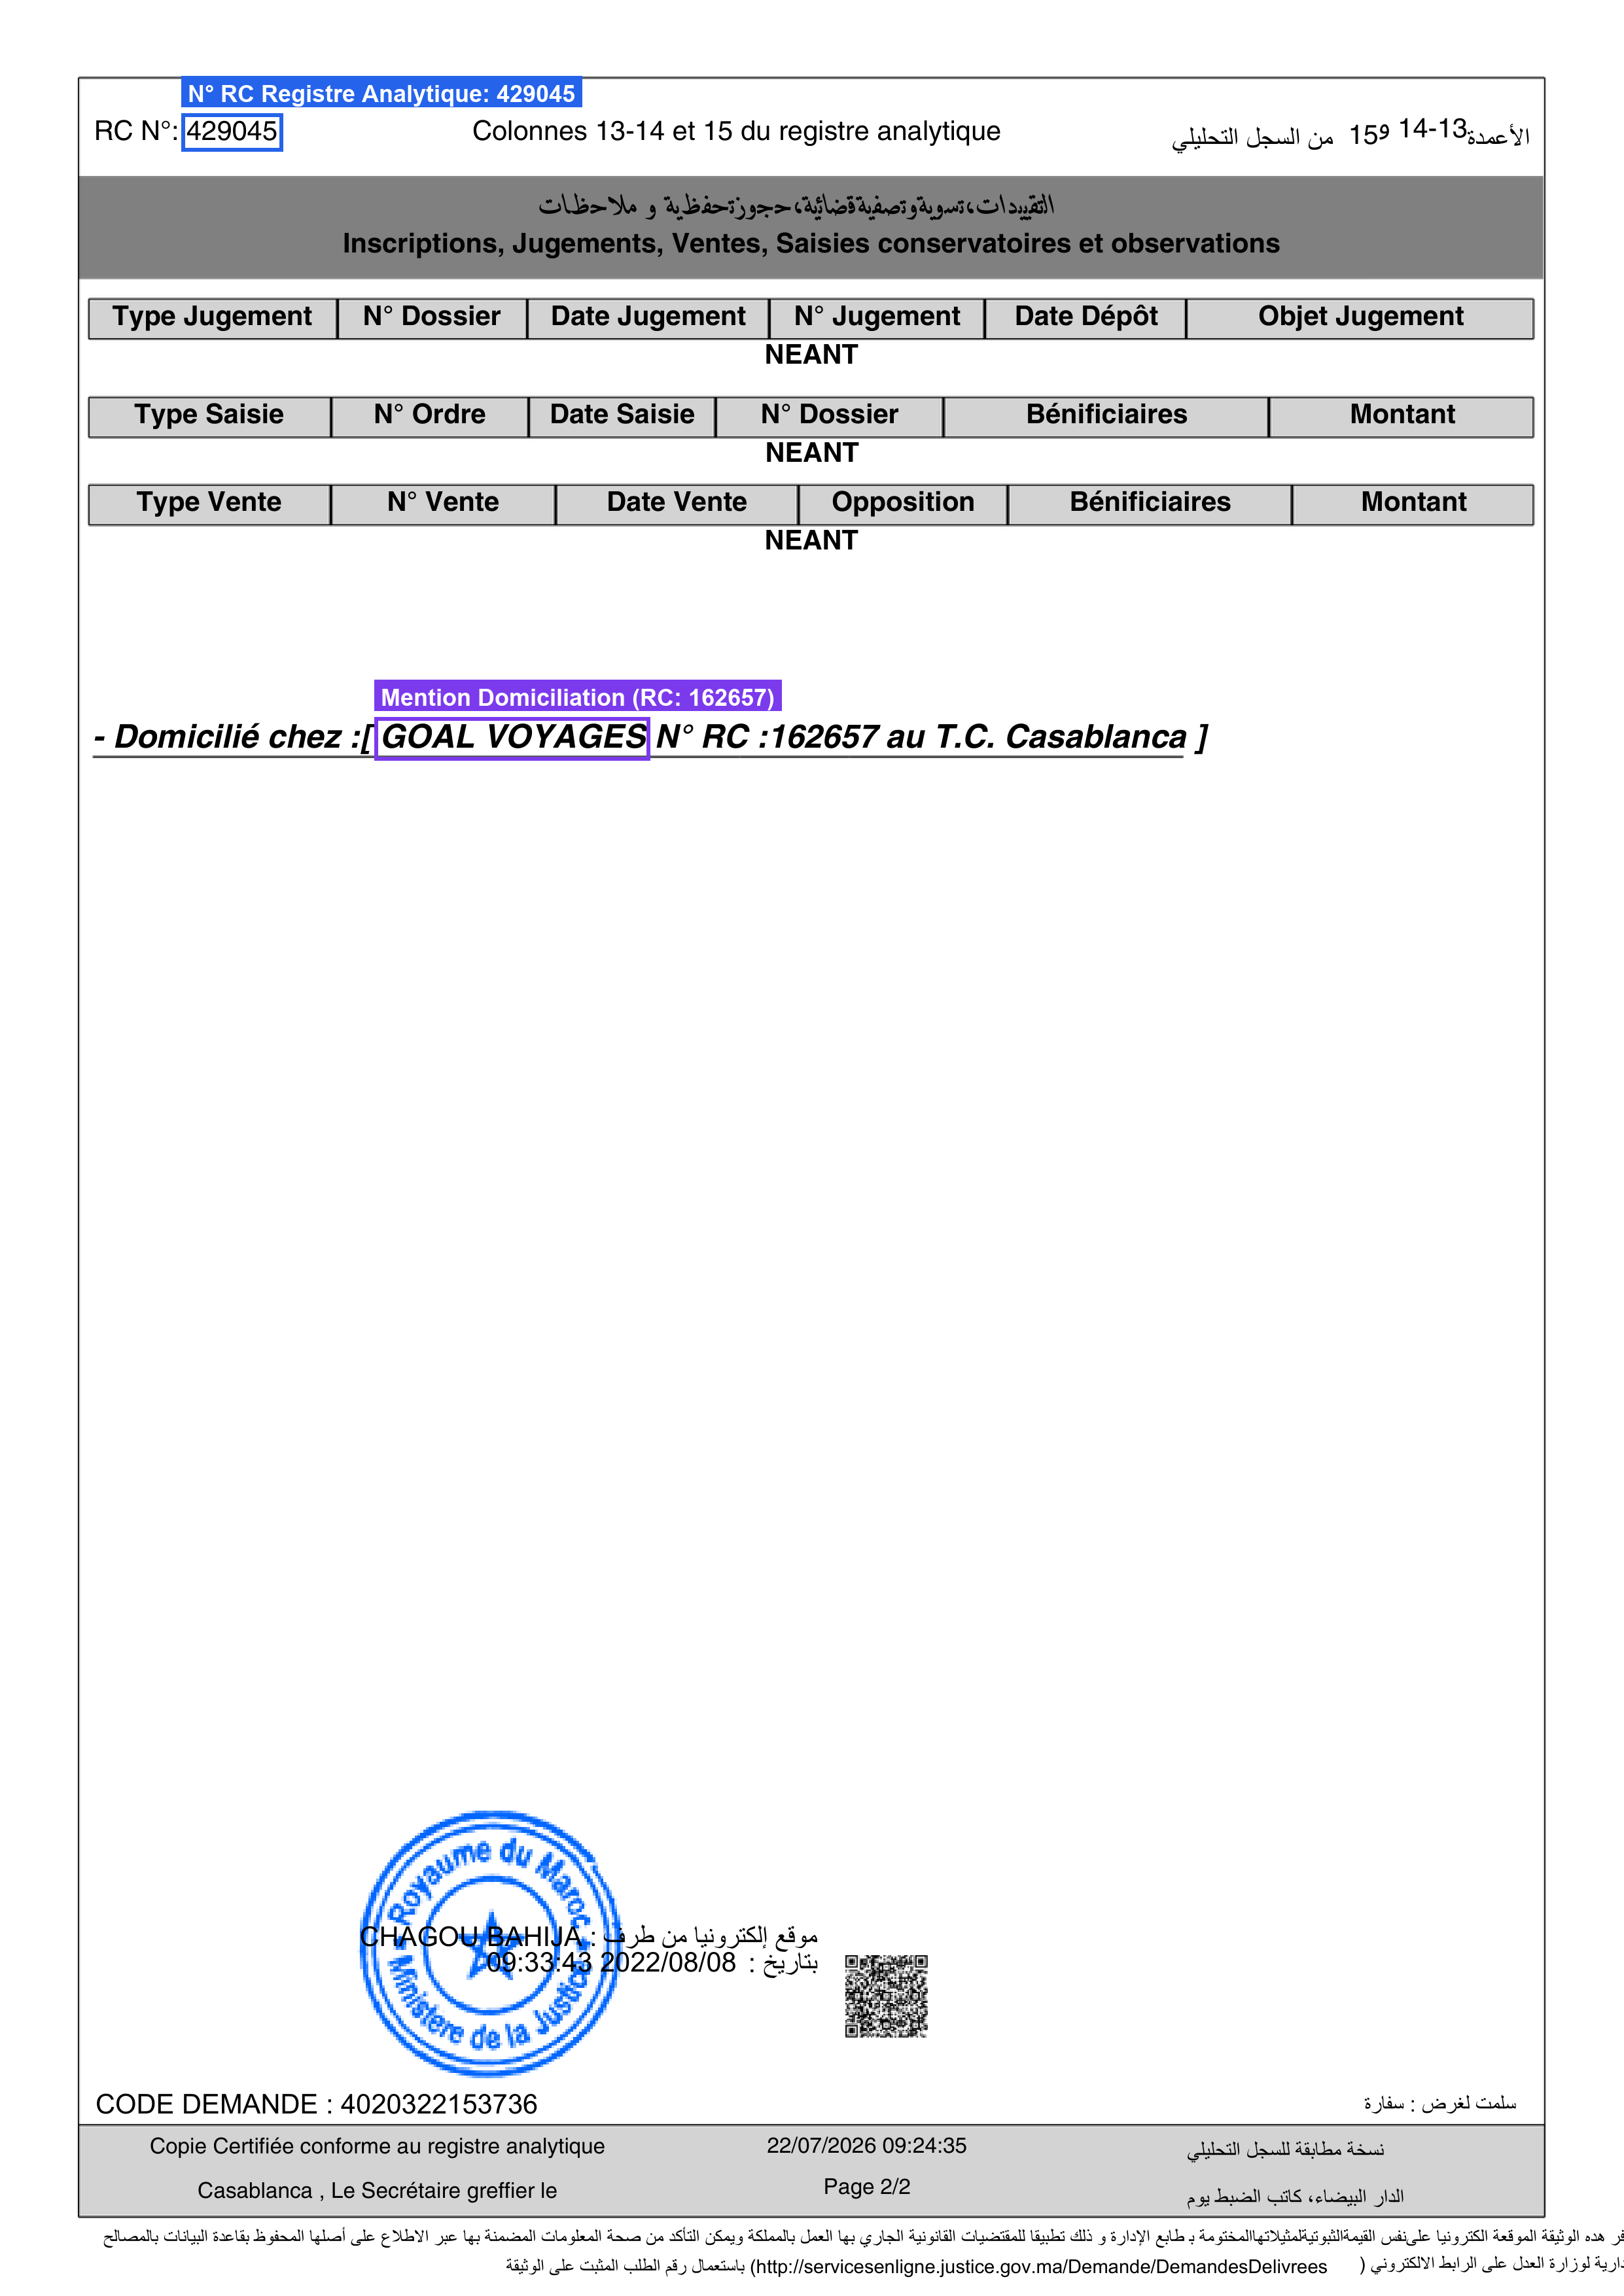
\includegraphics[width=0.72\textwidth]{Screenshots/model_j_page2_annotated.png}
    }{\IfFileExists{Screenshots/model_j_page2_clean.png}{
        \includegraphics[width=0.72\textwidth]{Screenshots/model_j_page2_clean.png}
    }{
        \fbox{\parbox{12cm}{\centering\vspace{2.5cm}\textit{Échantillon Mod\`{e}le J (Page 2)}\vspace{2.5cm}}}
    }}
    \caption{Page 2 du Mod\`{e}le J : Identification du Registre Analytique et de la mention de Domiciliation (\texttt{GOAL VOYAGES N° RC : 162657}).}
    \label{fig:model-j-page2-annotated}
\end{figure}

\begin{figure}[H]
    \centering
    \IfFileExists{Screenshots/document_if_annotated.png}{
        
\includegraphics[width=0.72\textwidth]{Screenshots/document_if_annotated.png}
    }{\IfFileExists{Screenshots/document_if_clean.png}{
        \includegraphics[width=0.72\textwidth]{Screenshots/document_if_clean.png}
    }{
        \fbox{\parbox{12cm}{\centering\vspace{2.5cm}\textit{Échantillon Document IF}\vspace{2.5cm}}}
    }}
    \caption{Bo\^{\i}tes englobantes d'extraction d'entit\'{e}s sur le Bulletin de Notification Identifiant Fiscal (IF) avec mise en valeur de l'IF (\texttt{32770927}).}
    \label{fig:doc-if-annotated}
\end{figure}

\begin{figure}[H]
    \centering
    \IfFileExists{Screenshots/ice_cert_annotated.png}{
        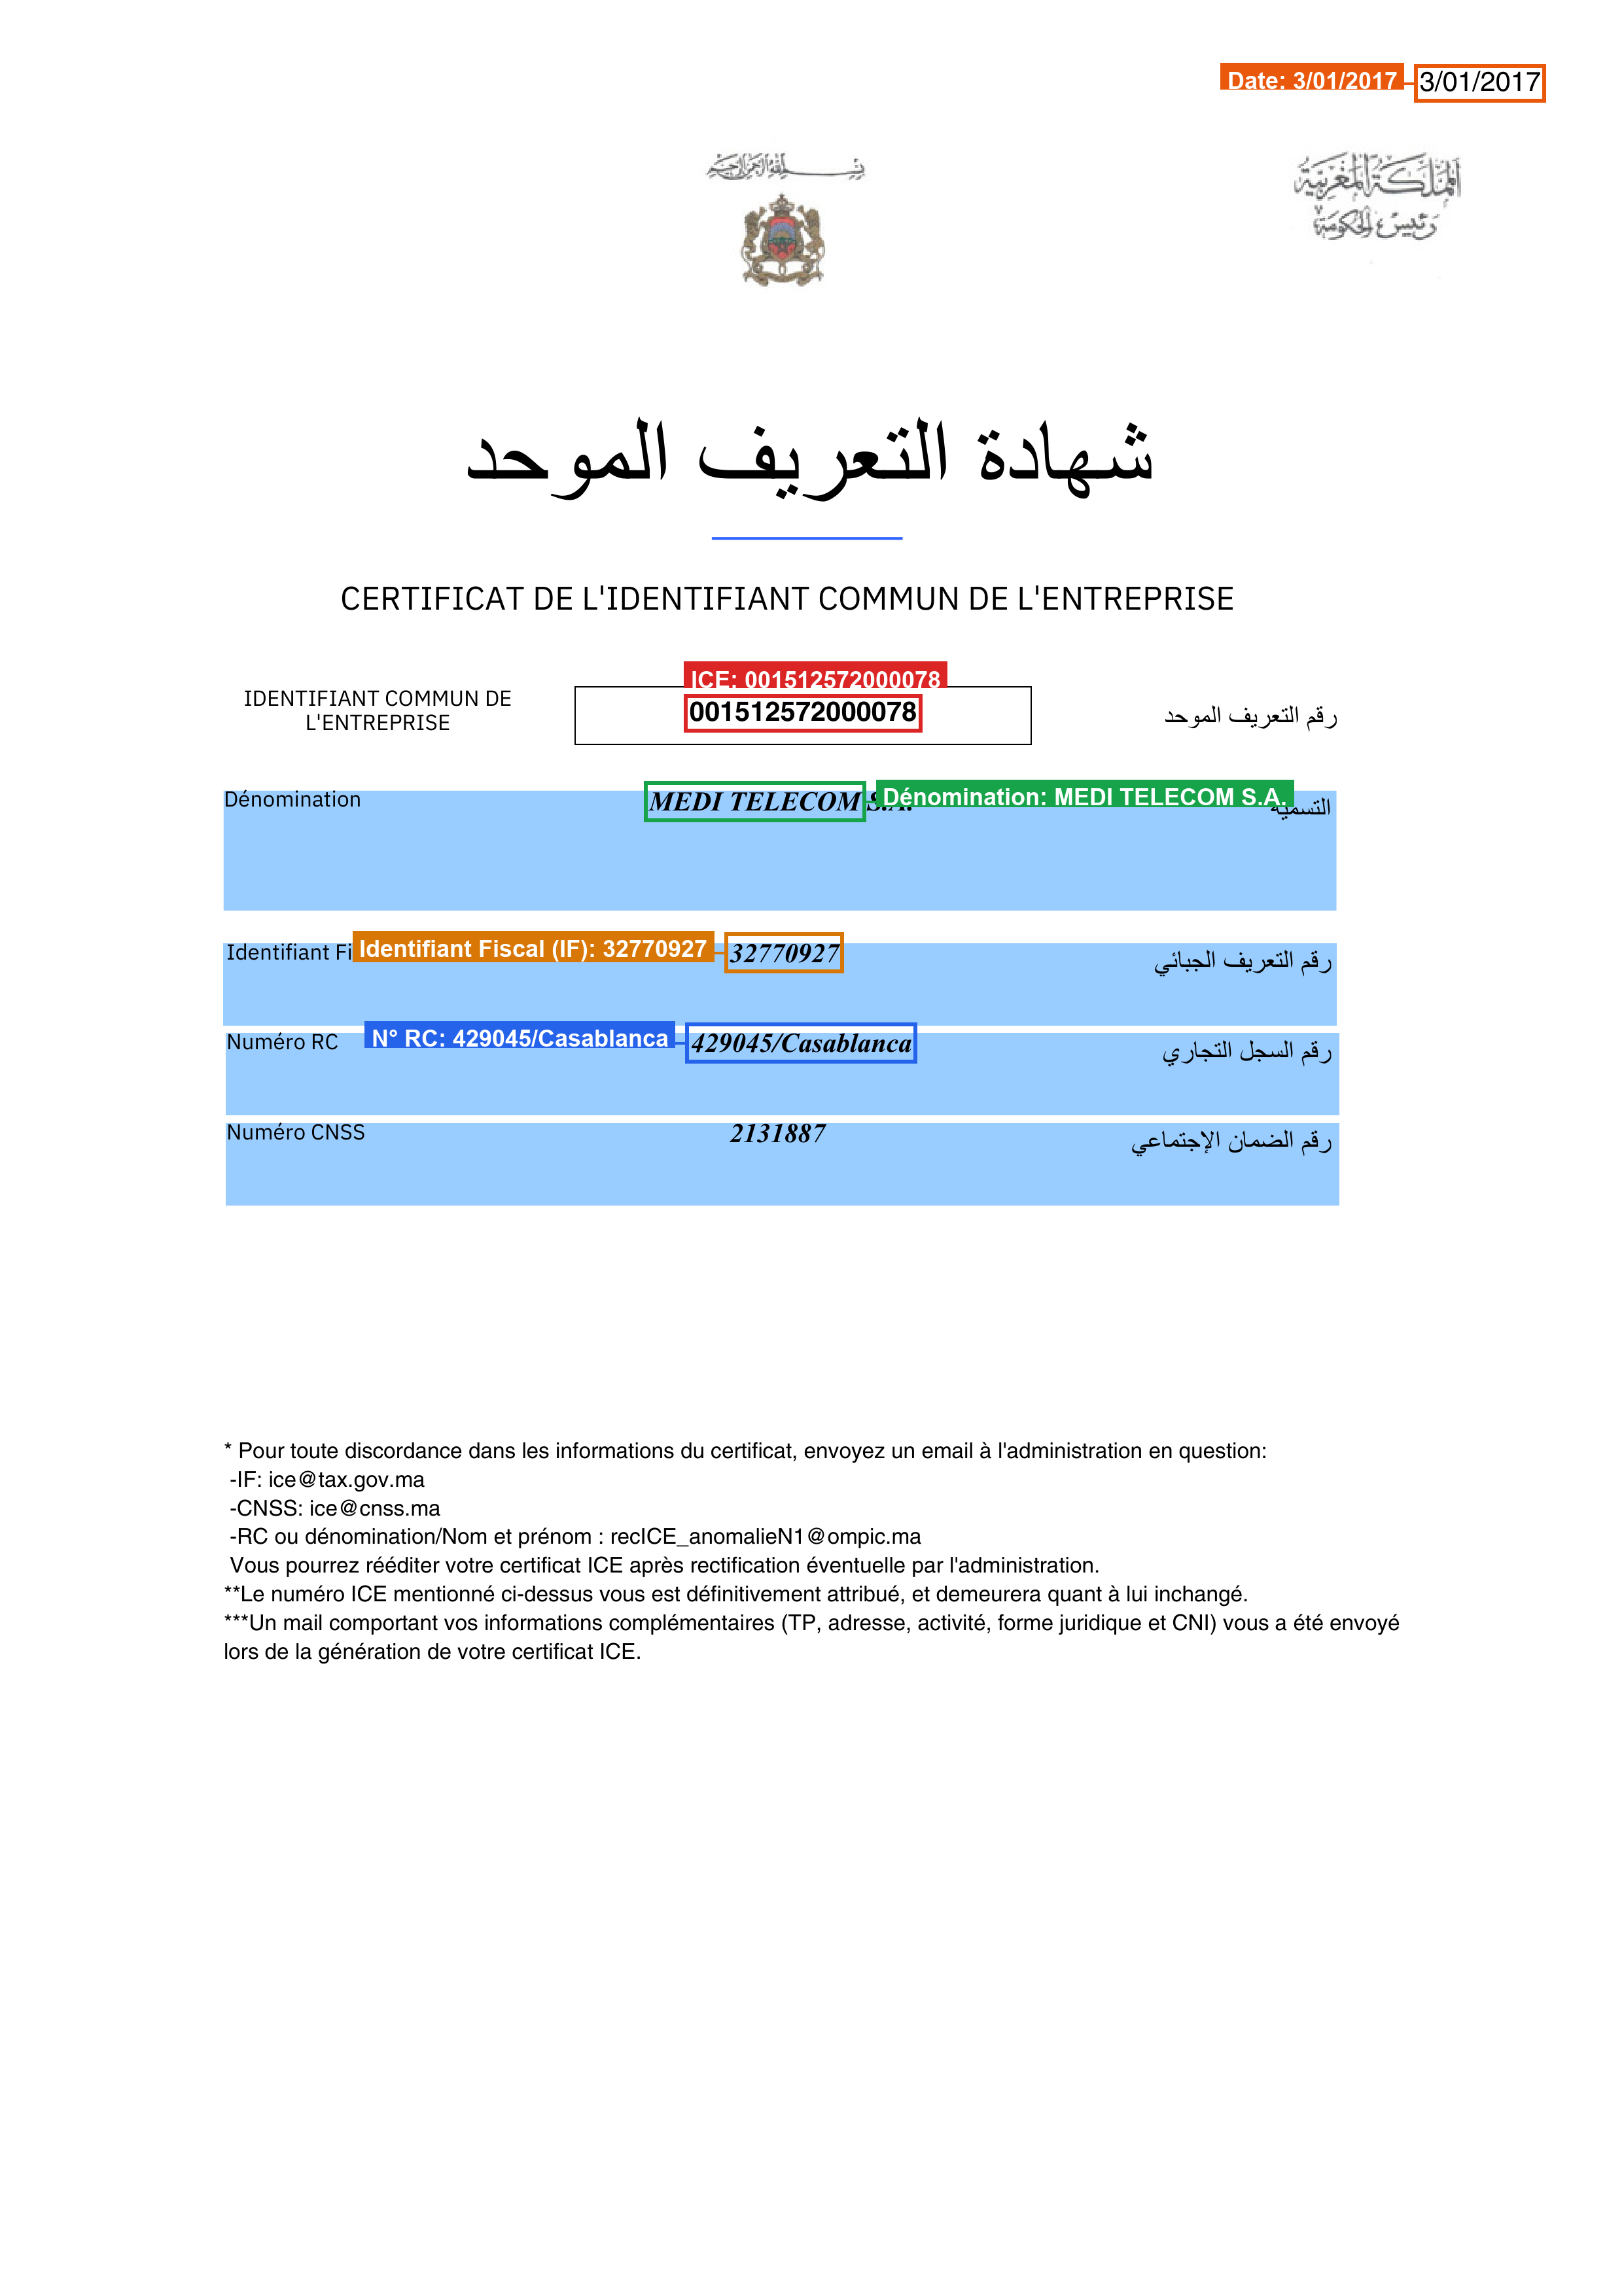
\includegraphics[width=0.72\textwidth]{Screenshots/ice_cert_annotated.png}
    }{\IfFileExists{Screenshots/ice_cert_clean.png}{
        \includegraphics[width=0.72\textwidth]{Screenshots/ice_cert_clean.png}
    }{
        \fbox{\parbox{12cm}{\centering\vspace{2.5cm}\textit{Échantillon Certificat ICE}\vspace{2.5cm}}}
    }}
    \caption{Zones d'extraction d'entit\'{e}s sur la Page 1 du Certificat d'Identifiant Commun de l'Entreprise (ICE).}
    \label{fig:ice-cert-annotated}
\end{figure}

\begin{figure}[H]
    \centering
    \IfFileExists{Screenshots/taxe_pro_annotated.png}{
        
\includegraphics[width=0.72\textwidth]{Screenshots/taxe_pro_annotated.png}
    }{\IfFileExists{Screenshots/taxe_pro_clean.png}{
        \includegraphics[width=0.72\textwidth]{Screenshots/taxe_pro_clean.png}
    }{
        \fbox{\parbox{12cm}{\centering\vspace{2.5cm}\textit{Échantillon Taxe Professionnelle}\vspace{2.5cm}}}
    }}
    \caption{Bo\^{\i}tes englobantes d'extraction sur le Bulletin de Taxe Professionnelle (TP).}
    \label{fig:taxe-pro-annotated}
\end{figure}

\begin{figure}[H]
    \centering
    \IfFileExists{Screenshots/domiciliation_annotated.png}{
        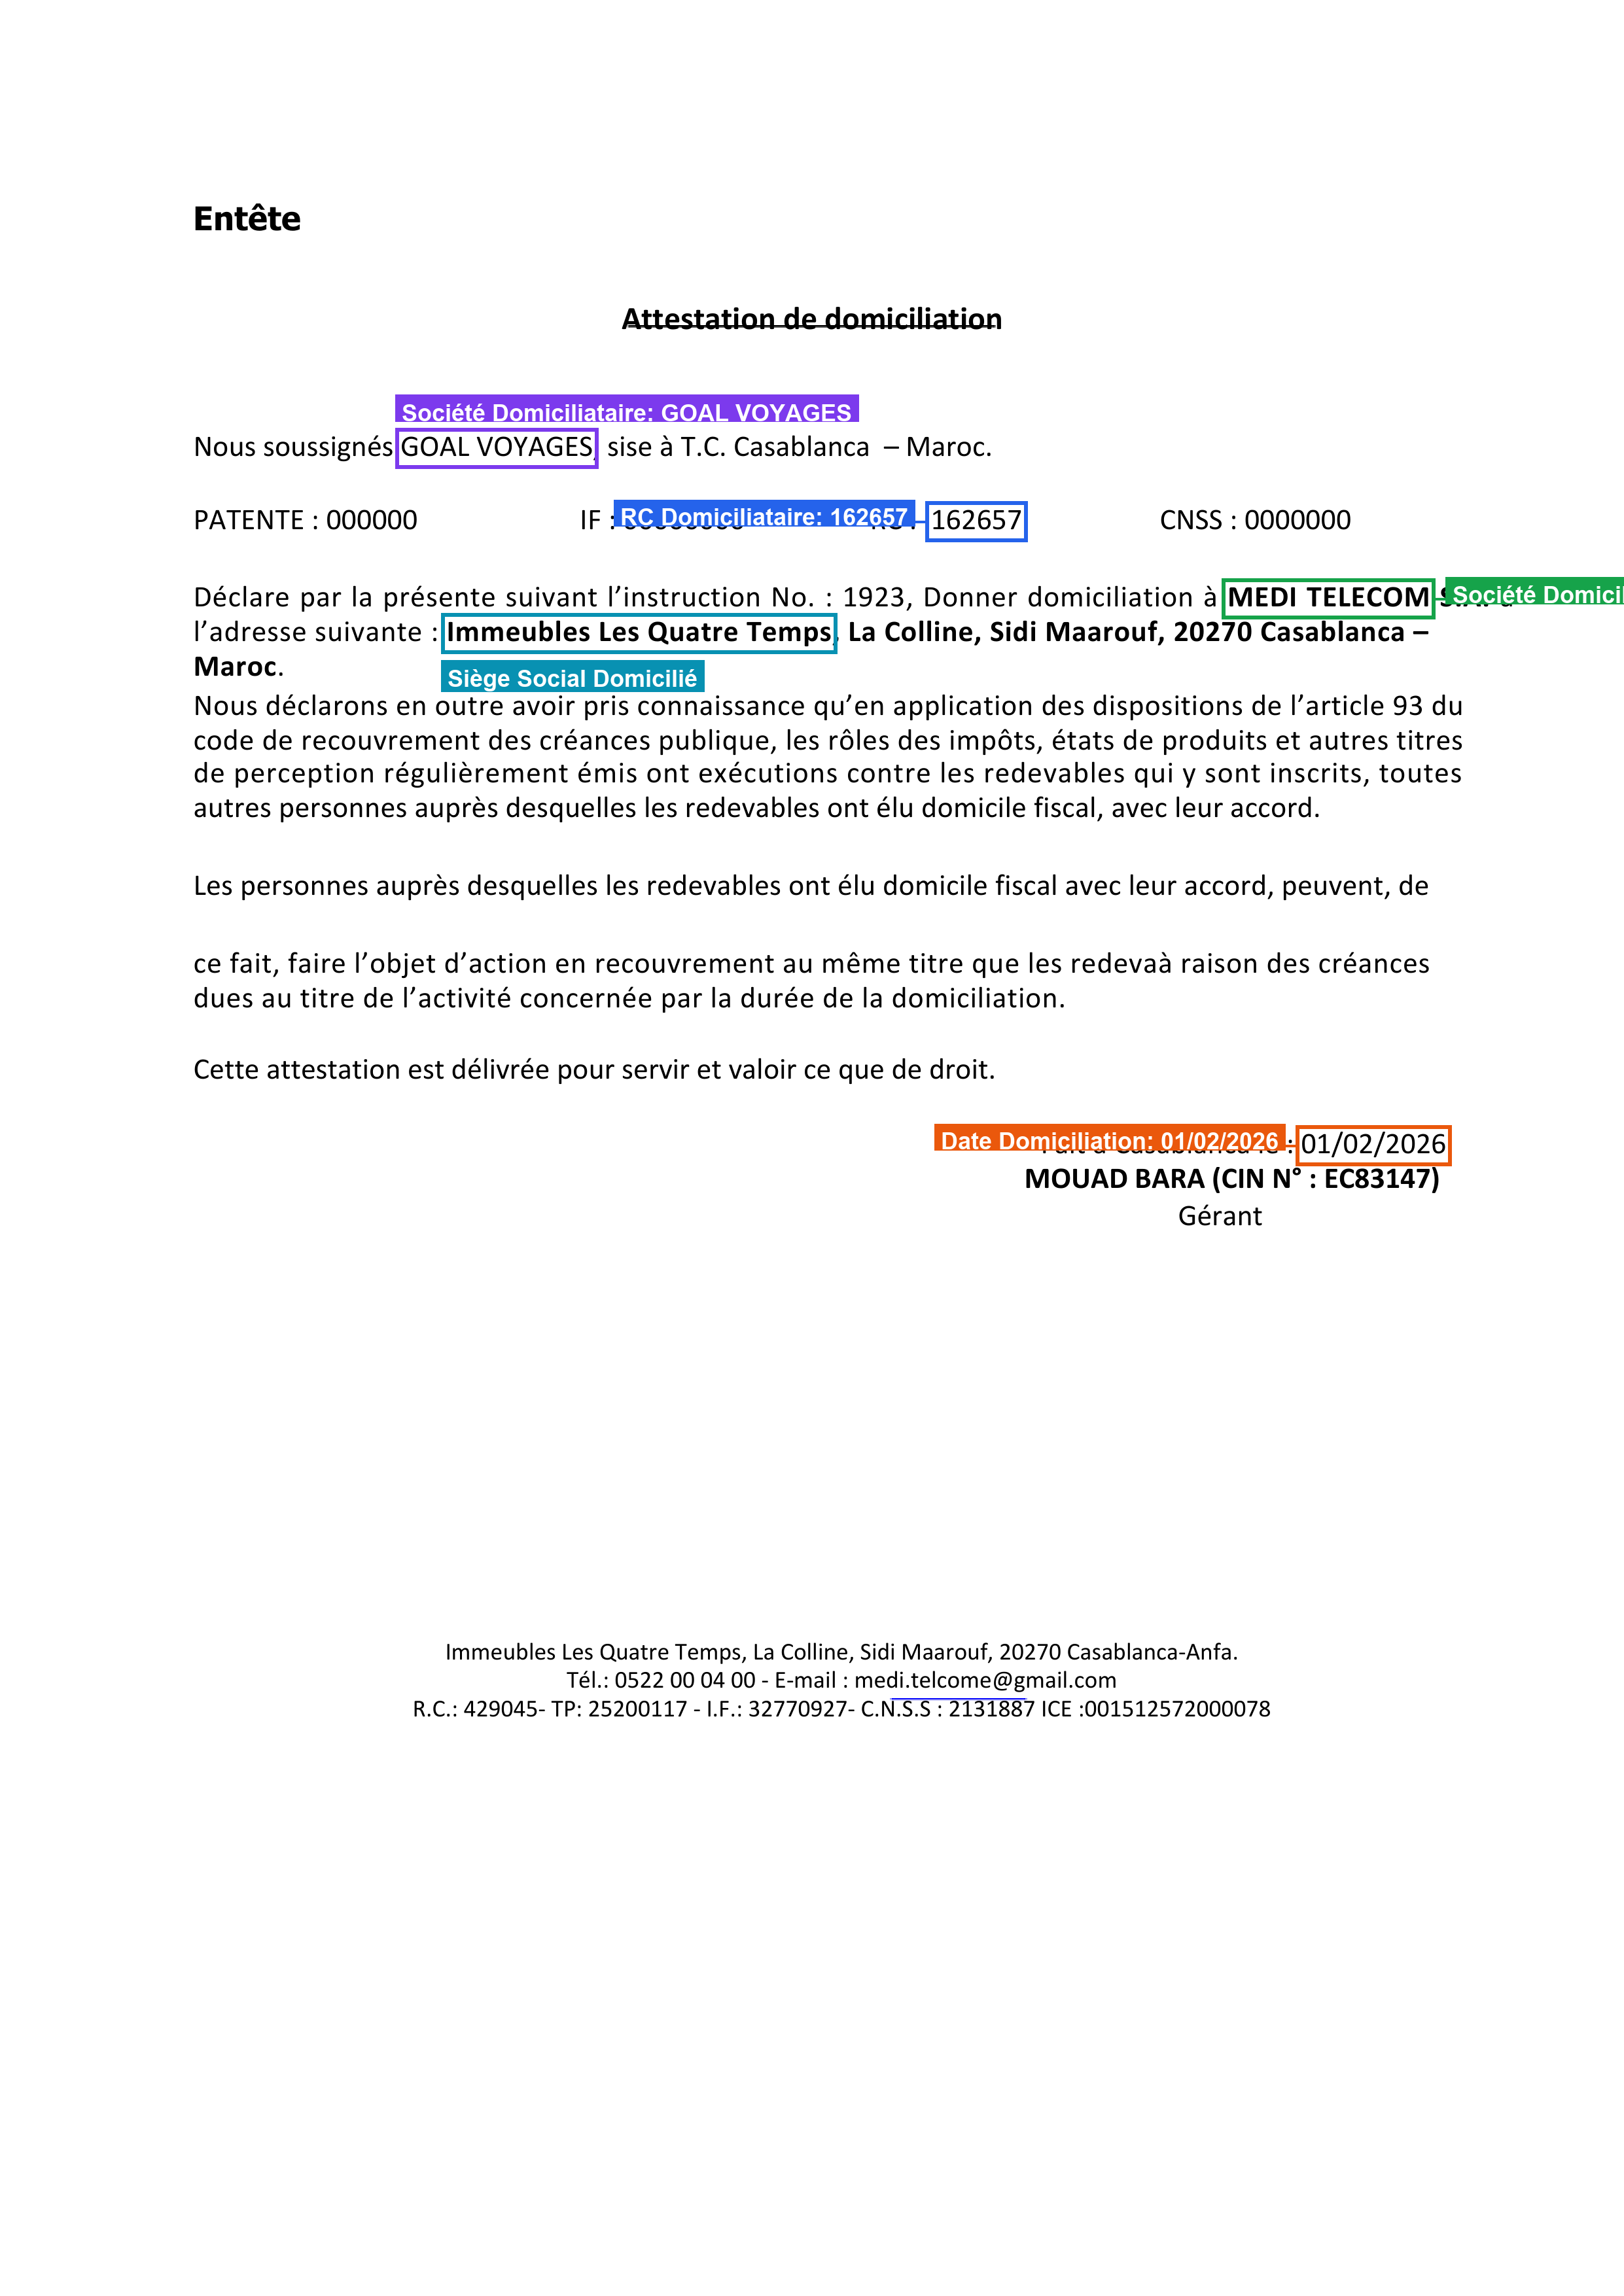
\includegraphics[width=0.72\textwidth]{Screenshots/domiciliation_annotated.png}
    }{\IfFileExists{Screenshots/domiciliation_clean.png}{
        \includegraphics[width=0.72\textwidth]{Screenshots/domiciliation_clean.png}
    }{
        \fbox{\parbox{12cm}{\centering\vspace{2.5cm}\textit{Échantillon Domiciliation}\vspace{2.5cm}}}
    }}
    \caption{Zones d'extraction de l'Attestation de Domiciliation Commerciale : Cross-référence avec la Page 2 du Mod\`{e}le J (\texttt{GOAL VOYAGES N° RC : 162657}).}
    \label{fig:domiciliation-annotated}
\end{figure}

\begin{figure}[H]
    \centering
    \IfFileExists{Screenshots/cni_annotated.png}{
        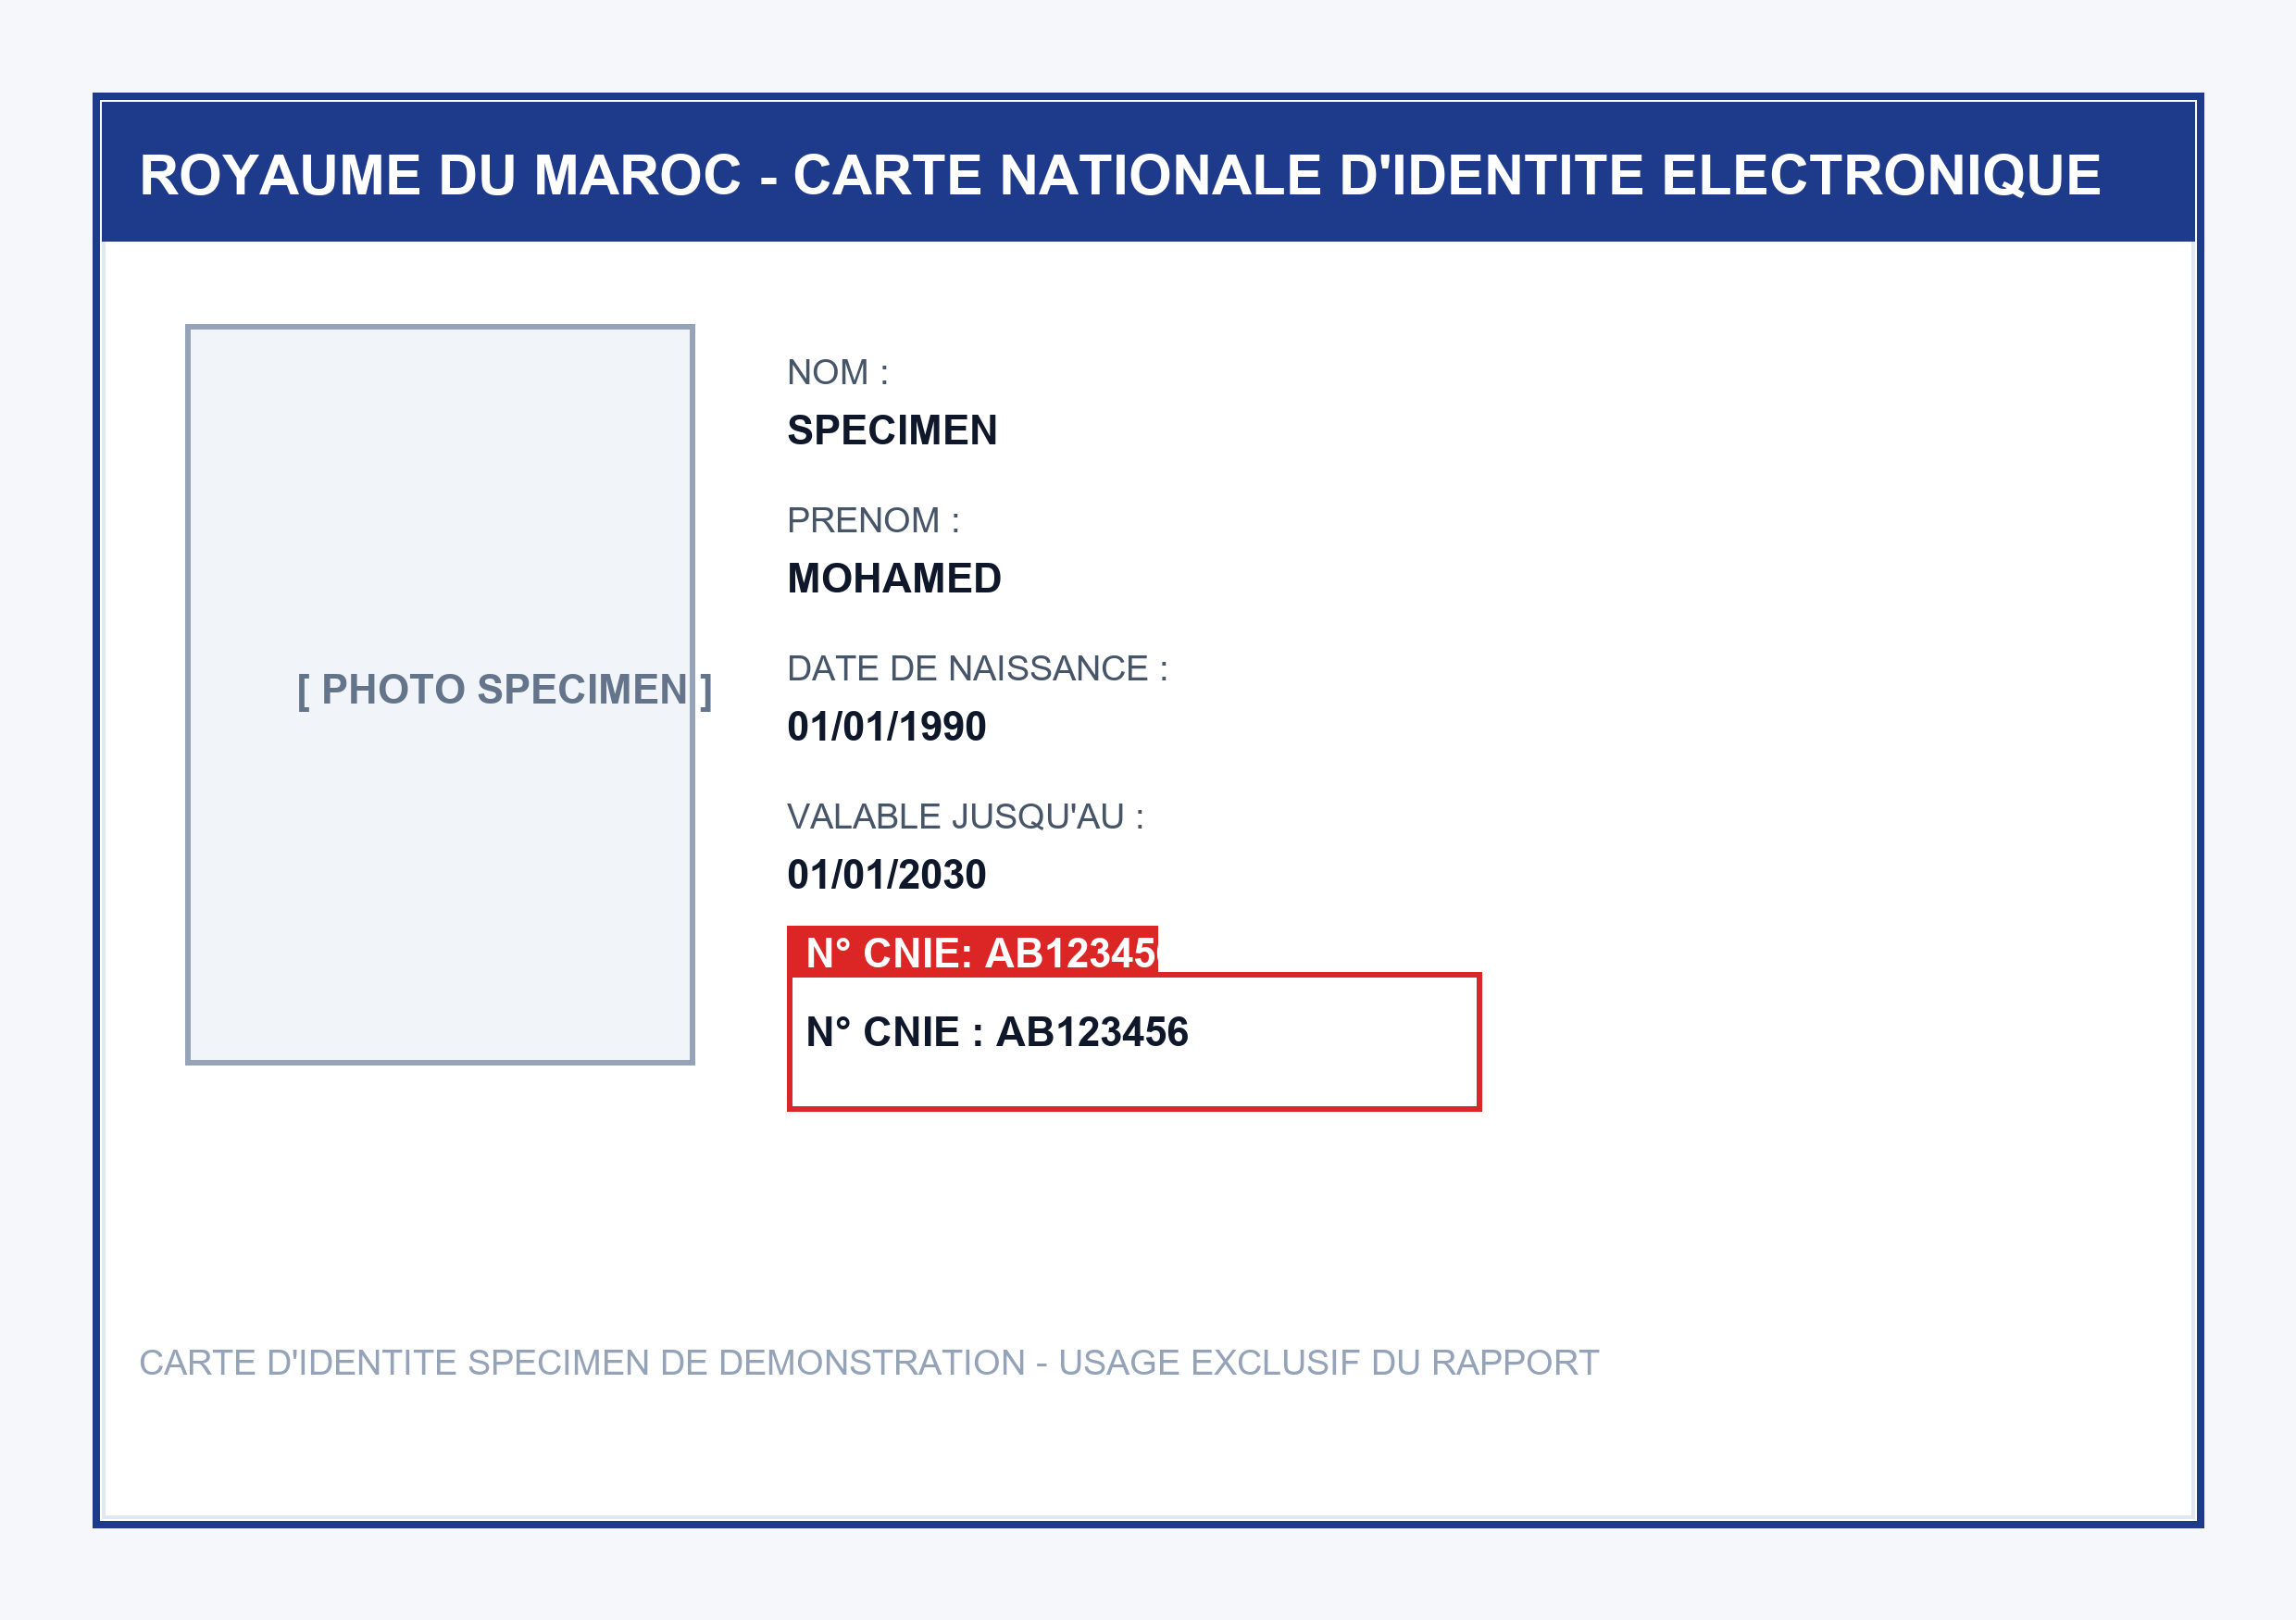
\includegraphics[width=0.72\textwidth]{Screenshots/cni_annotated.png}
    }{\IfFileExists{Screenshots/cni_clean.png}{
        \includegraphics[width=0.72\textwidth]{Screenshots/cni_clean.png}
    }{
        \fbox{\parbox{12cm}{\centering\vspace{2.5cm}\textit{Échantillon CNIE}\vspace{2.5cm}}}
    }}
    \caption{Zones d'extraction de la Carte Nationale d'Identit\'{e} \'{E}lectronique (CNIE) : Point d'ancrage g\'{e}rant (\textsc{BOUALAM MOHAMED}, \texttt{AB123456}).}
    \label{fig:cni-annotated}
\end{figure}

\section{Validation Modulo~97}

\subsection{Validation du RIB}

L'algorithme de validation du RIB impl\'{e}mente la norme ISO~7064 avec support des RIB alphanum\'{e}riques :

\begin{lstlisting}[language=Python, caption={Validation RIB Modulo~97 (checksum.py).}, label={lst:validate-rib}]
_RIB_LETTER_MAP = {
    'A': '1', 'J': '1',
    'B': '2', 'K': '2', 'S': '2',
    'C': '3', 'L': '3', 'T': '3',
    # ... (table complete)
}

def validate_rib(rib: str) -> bool:
    """Validate 24-char Moroccan RIB using mod 97."""
    clean = re.sub(r'[\s\-]', '', rib).upper()
    rib_numeric = ''.join(
        _RIB_LETTER_MAP.get(c, c) for c in clean
    )
    if len(rib_numeric) != 24 or not rib_numeric.isdigit():
        return False
    return int(rib_numeric) % 97 == 0
\end{lstlisting}

\begin{figure}[H]
    \centering
    \IfFileExists{Screenshots/statuts_annotated.png}{
        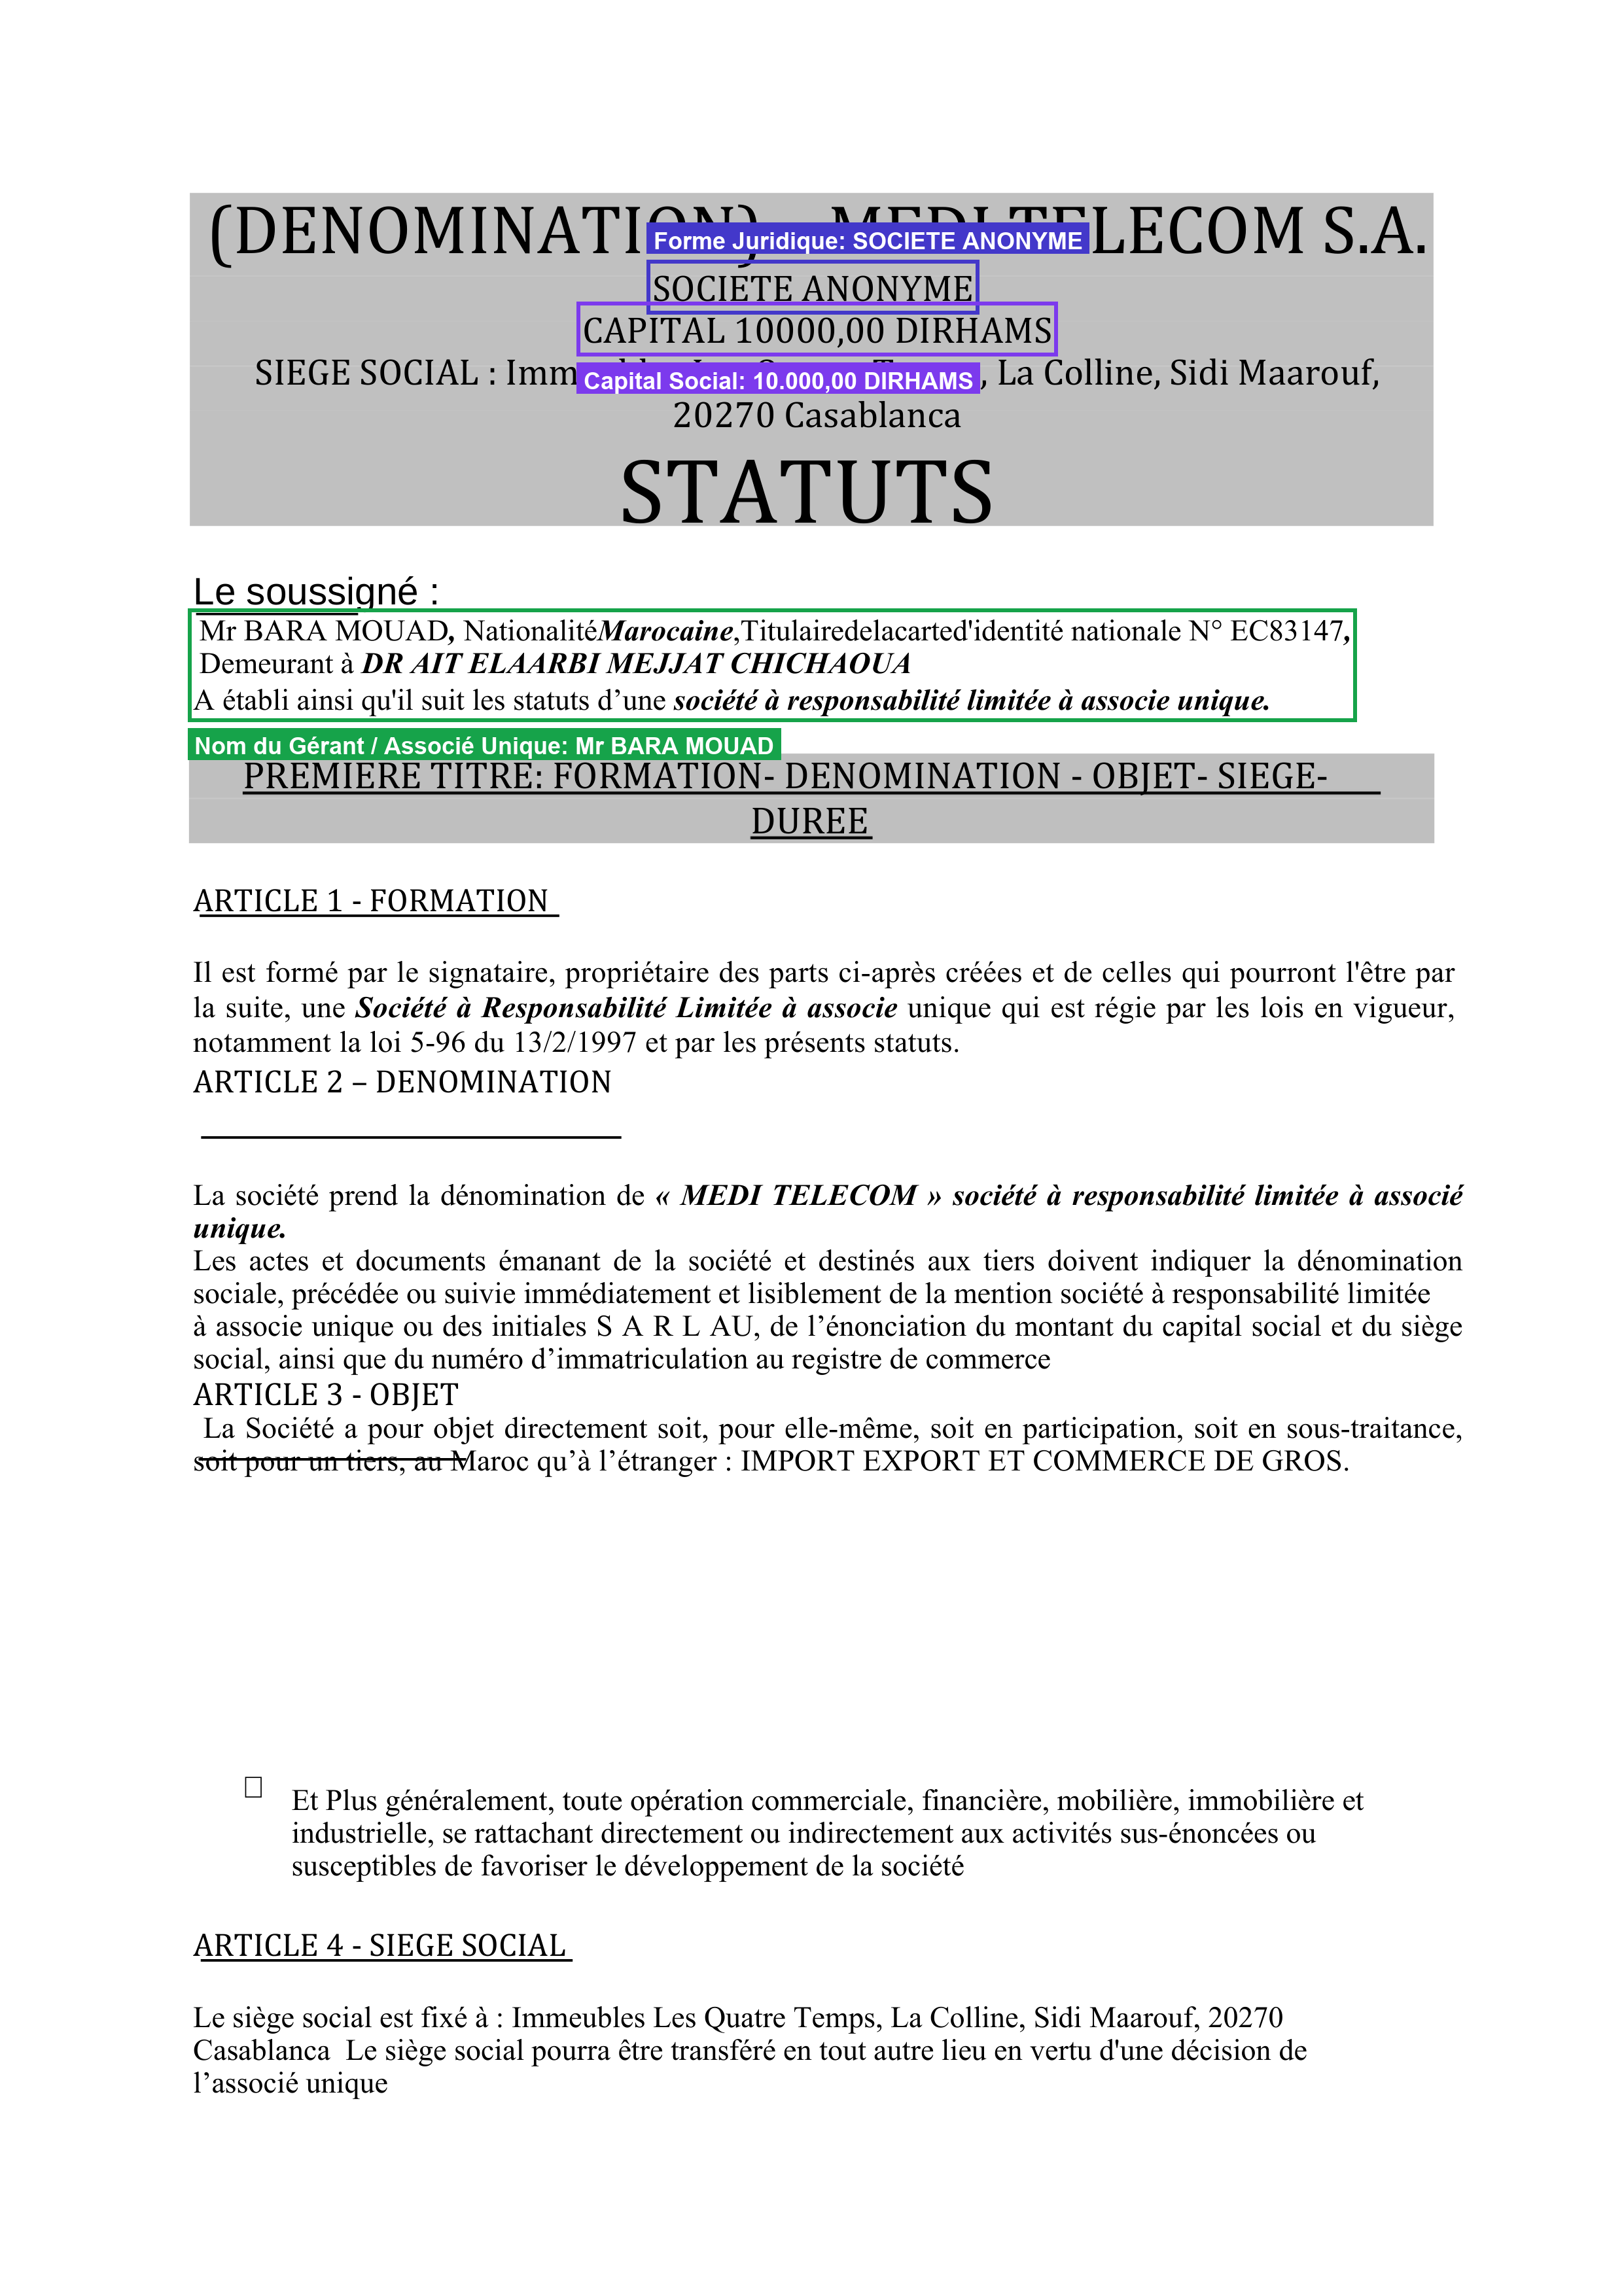
\includegraphics[width=0.72\textwidth]{Screenshots/statuts_annotated.png}
    }{
        \fbox{\parbox{12cm}{\centering\vspace{2.5cm}\textit{Échantillon Statuts de la Société avec rects d'extraction}\vspace{2.5cm}}}
    }
    \caption{Bo\^{\i}tes englobantes d'extraction sur la premi\`{e}re page des Statuts de la Soci\'{e}t\'{e}.}
    \label{fig:statuts-annotated}
\end{figure}

\begin{figure}[H]
    \centering
    \IfFileExists{Screenshots/rib_annotated.png}{
        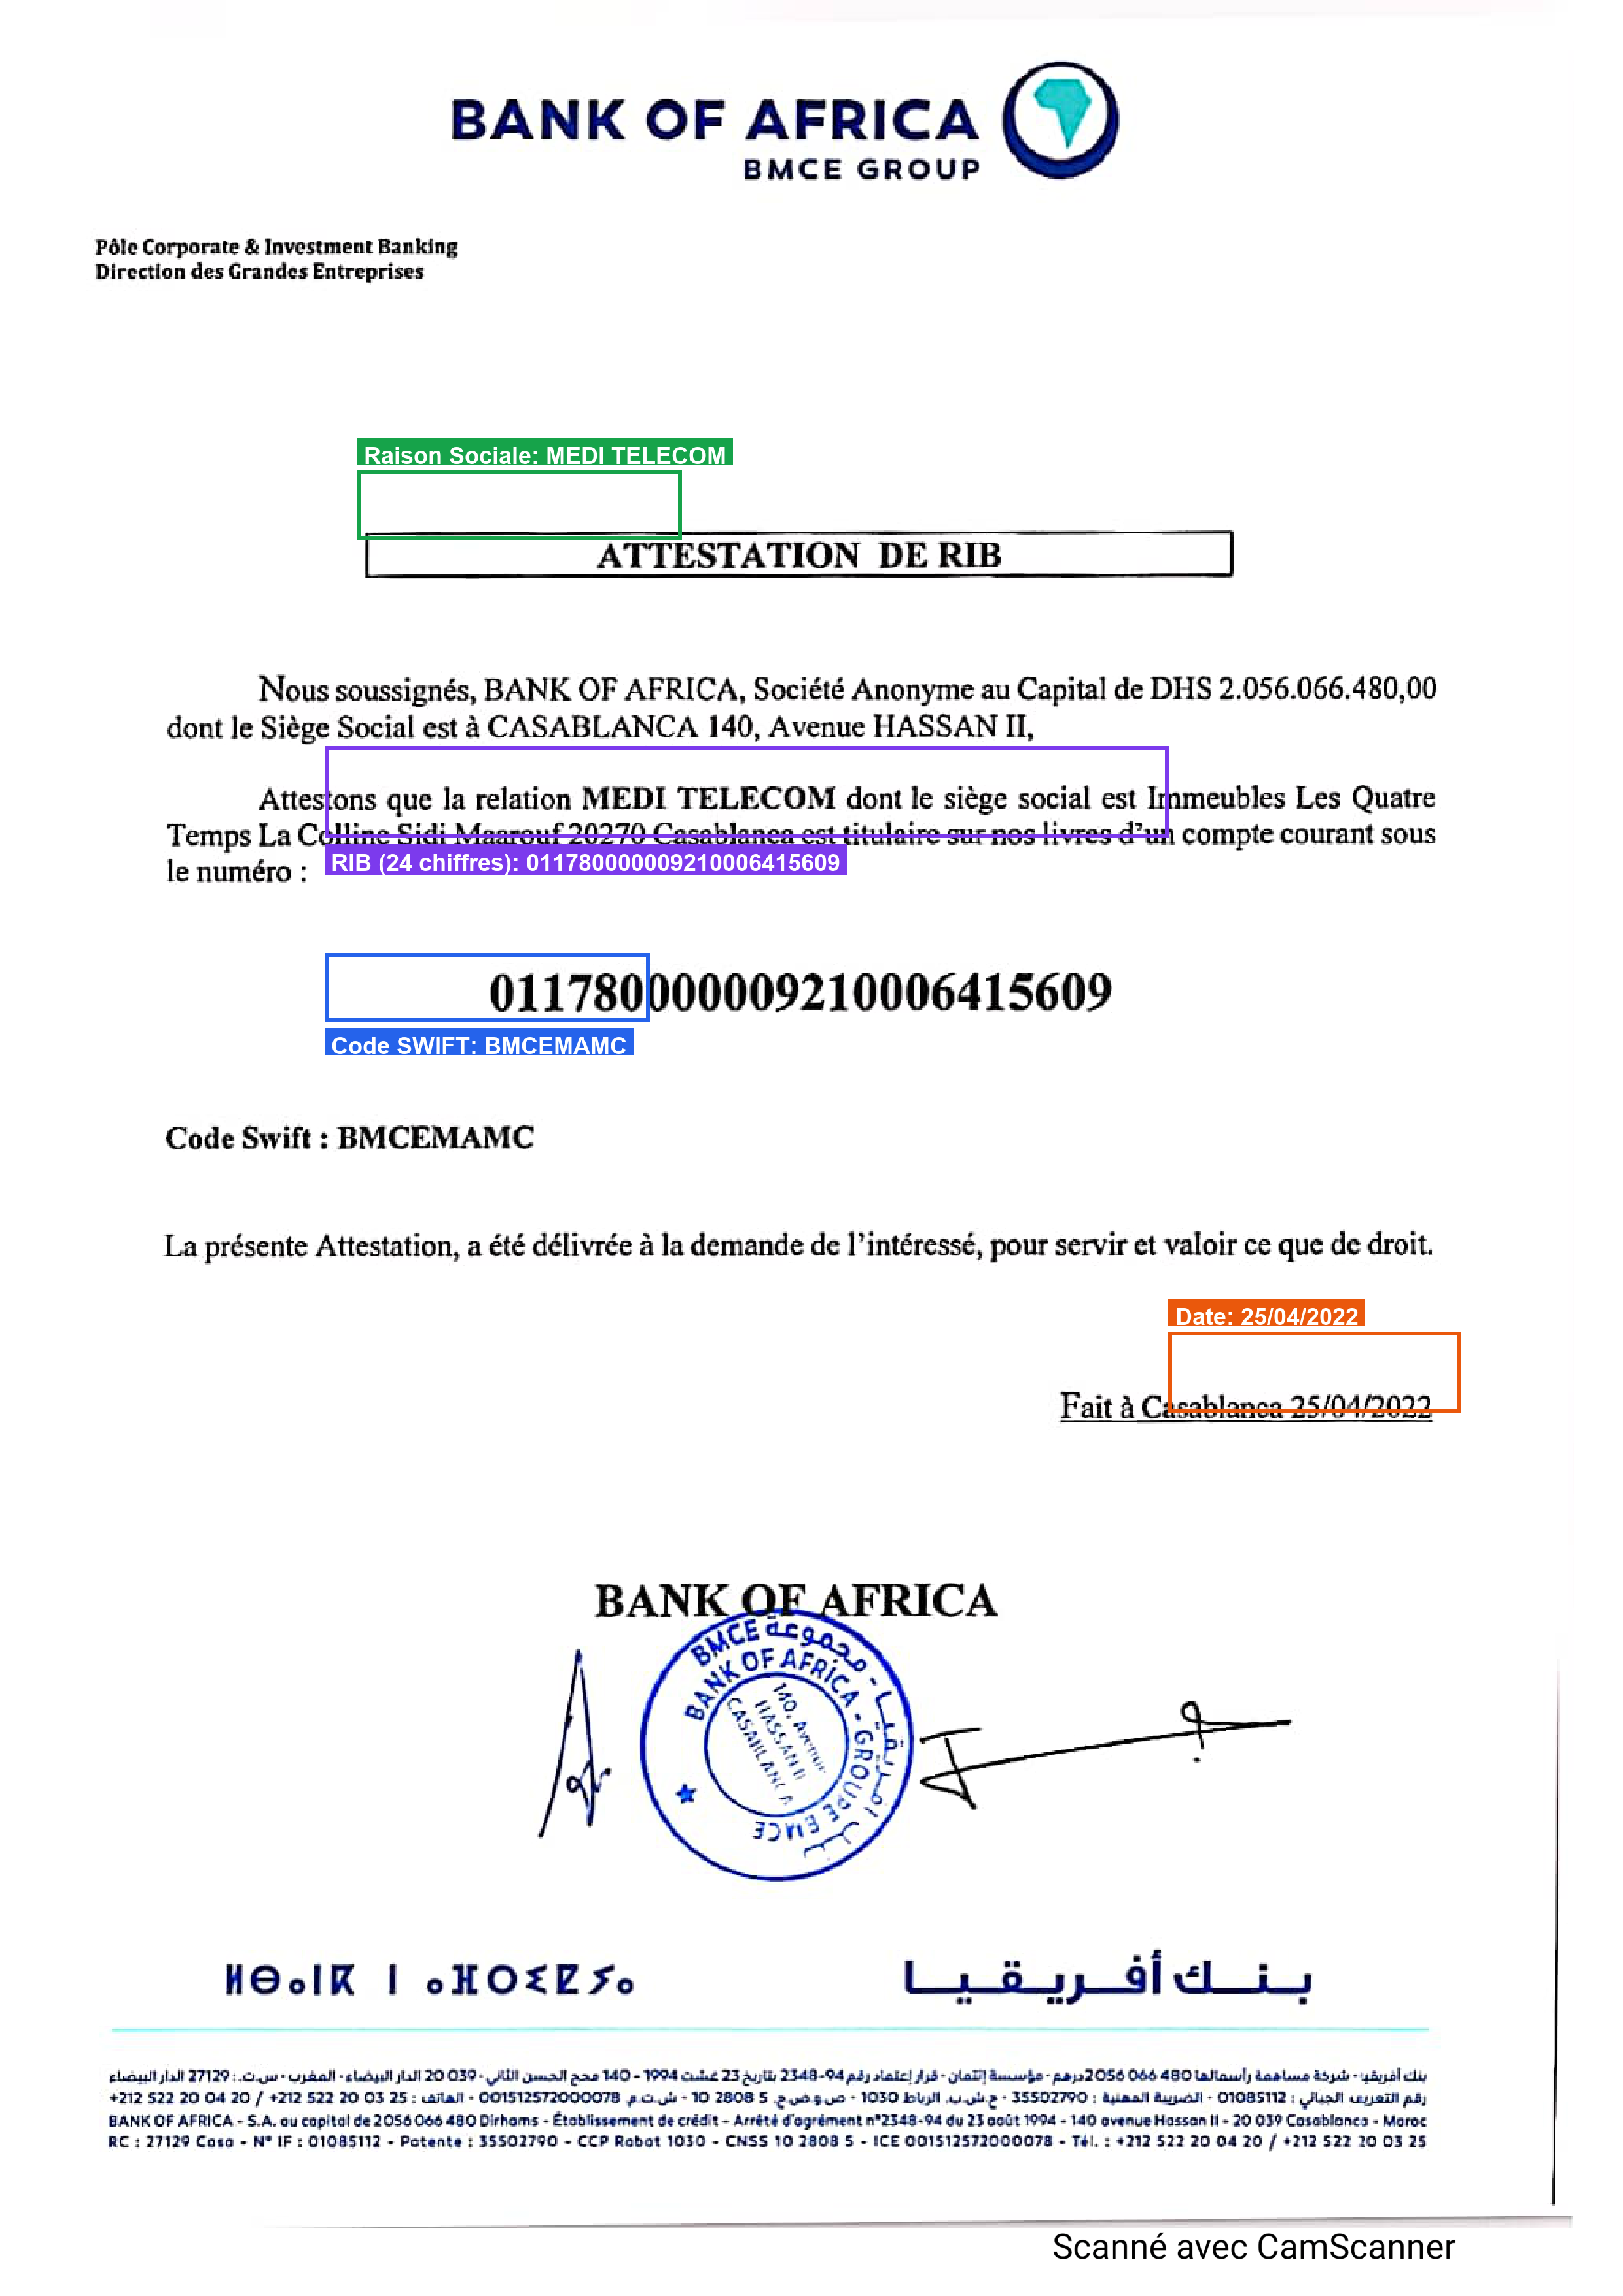
\includegraphics[width=0.72\textwidth]{Screenshots/rib_annotated.png}
    }{
        \fbox{\parbox{12cm}{\centering\vspace{2.5cm}\textit{Échantillon Attestation RIB avec rectangle d'extraction (24 chiffres)}\vspace{2.5cm}}}
    }
    \caption{Zone d'extraction du Relev\'{e} d'Identit\'{e} Bancaire (RIB 24 chiffres) soumis au contr\^{o}le Modulo~97.}
    \label{fig:rib-annotated}
\end{figure}

\subsection{Validation de l'ICE}

\begin{lstlisting}[language=Python, caption={Validation ICE Modulo~97 (checksum.py).}, label={lst:validate-ice}]
def validate_ice(ice: str) -> bool:
    """Validate 15-digit Moroccan ICE."""
    clean_ice = re.sub(r'[\s\-]', '', ice)
    if len(clean_ice) != 15 or not clean_ice.isdigit():
        return False
    base = int(clean_ice[:13])
    actual_key = int(clean_ice[13:15])
    computed_key = 97 - ((base * 100) % 97)
    if computed_key == 97:
        computed_key = 0  # Edge case
    return computed_key == actual_key
\end{lstlisting}

\begin{figure}[H]
    \centering
    \IfFileExists{images/modulo97_ice.png}{\includegraphics[width=0.9\textwidth]{images/modulo97_ice.png}}{\fbox{\parbox{12cm}{\centering\vspace{2cm}\textit{Algorithme Modulo~97 ICE --- Exporter depuis modulo97\_ice.drawio}\vspace{2cm}}}}
    \caption{Sch\'{e}ma de l'algorithme de validation Modulo~97 pour l'ICE (15 chiffres).}
    \label{fig:modulo97-ice}
\end{figure}

\subsection{V\'{e}rification MRZ (CNIE)}

\begin{lstlisting}[language=Python, caption={Calcul du chiffre de contr\^{o}le MRZ ICAO (checksum.py).}, label={lst:mrz-check}]
def calculate_mrz_check_digit(data: str) -> int:
    """ICAO Doc 9303 check digit: weights [7,3,1]."""
    WEIGHTS = [7, 3, 1]
    def char_val(c):
        if c.isdigit(): return int(c)
        elif c.isalpha(): return ord(c.upper()) - 55
        elif c == '<': return 0
    total = sum(
        char_val(c) * WEIGHTS[i % 3]
        for i, c in enumerate(data)
    )
    return total % 10
\end{lstlisting}

\section{Moteur de Cross-R\'{e}f\'{e}rence}

Le moteur de cross-r\'{e}f\'{e}rence compare syst\'{e}matiquement les variables extraites de chaque document avec les donn\'{e}es du formulaire. L'impl\'{e}mentation utilise trois strat\'{e}gies de comparaison :

\begin{lstlisting}[language=Python, caption={Cross-r\'{e}f\'{e}rence ICE (cross\_reference.py).}, label={lst:cross-ref-ice}]
def check_cross_consistency(form, docs):
    """Cross-checks extracted data against form."""
    checks = []
    overall_status = ValidationStatus.VALID
    
    # 1. ICE CROSS-REFERENCE (Strict matching)
    for doc_name, doc in docs.items():
        doc_ice = getattr(doc, 'ice', None)
        if doc_ice:
            is_match = doc_ice.strip() == form.ice.strip()
            status = (ValidationStatus.VALID if is_match
                      else ValidationStatus.INVALID)
            checks.append(FieldValidation(
                field_name="ICE",
                expected_value=form.ice,
                extracted_value=doc_ice,
                status=status,
                message=f"ICE {'match' if is_match else 'mismatch'}"
            ))
\end{lstlisting}

\begin{lstlisting}[language=Python, caption={Comparaison num\'{e}rique s\'{e}curis\'{e}e du RC (cross\_reference.py).}, label={lst:safe-numeric}]
def _safe_numeric_match(val1, val2):
    """Compare numeric strings by digits only.
    Handles '370621/CASABLANCA' vs '370621'."""
    digits1 = re.sub(r'\D', '', val1)
    digits2 = re.sub(r'\D', '', val2)
    if not digits1 or not digits2:
        return False
    return digits1.lstrip('0') == digits2.lstrip('0')
\end{lstlisting}

\section{Backend FastAPI}

Le backend expose deux endpoints REST :

\begin{lstlisting}[language=Python, caption={Backend FastAPI (app.py).}, label={lst:fastapi-app}]
app = FastAPI(title="Souscription API")

class Inscription(BaseModel):
    raison_sociale: Optional[str] = None
    ice: Optional[str] = None
    identifiant_fiscal: Optional[str] = None
    rc_numero: Optional[str] = None
    rc_ville: Optional[str] = None
    organisme: Optional[str] = None  # DOUANE | PORTNET_DOUANE
    gerants: Optional[list[Gerant]] = None

@app.post("/api/inscriptions")
def create_inscription(data: Inscription):
    """Enregistre une inscription dans PostgreSQL."""
    conn = psycopg2.connect(**DB)
    cur = conn.cursor()
    cur.execute("""
        INSERT INTO inscriptions
            (raison_sociale, ice, rc_numero, ...)
        VALUES (%s, %s, %s, ...)
        RETURNING id""",
        (data.raison_sociale, data.ice, ...))
    insc_id = cur.fetchone()[0]
    conn.commit()
    return {"ok": True, "id": str(insc_id)}
\end{lstlisting}

Apr\`{e}s la soumission, le backend persiste chaque document t\'{e}l\'{e}vers\'{e} dans un r\'{e}pertoire organis\'{e} par type de document, en lui attribuant un identifiant unique (GUID). La figure~\ref{fig:documents-stockes} illustre le tableau r\'{e}capitulatif des documents stock\'{e}s avec leurs m\'{e}tadonn\'{e}es.

\begin{figure}[H]
    \centering
    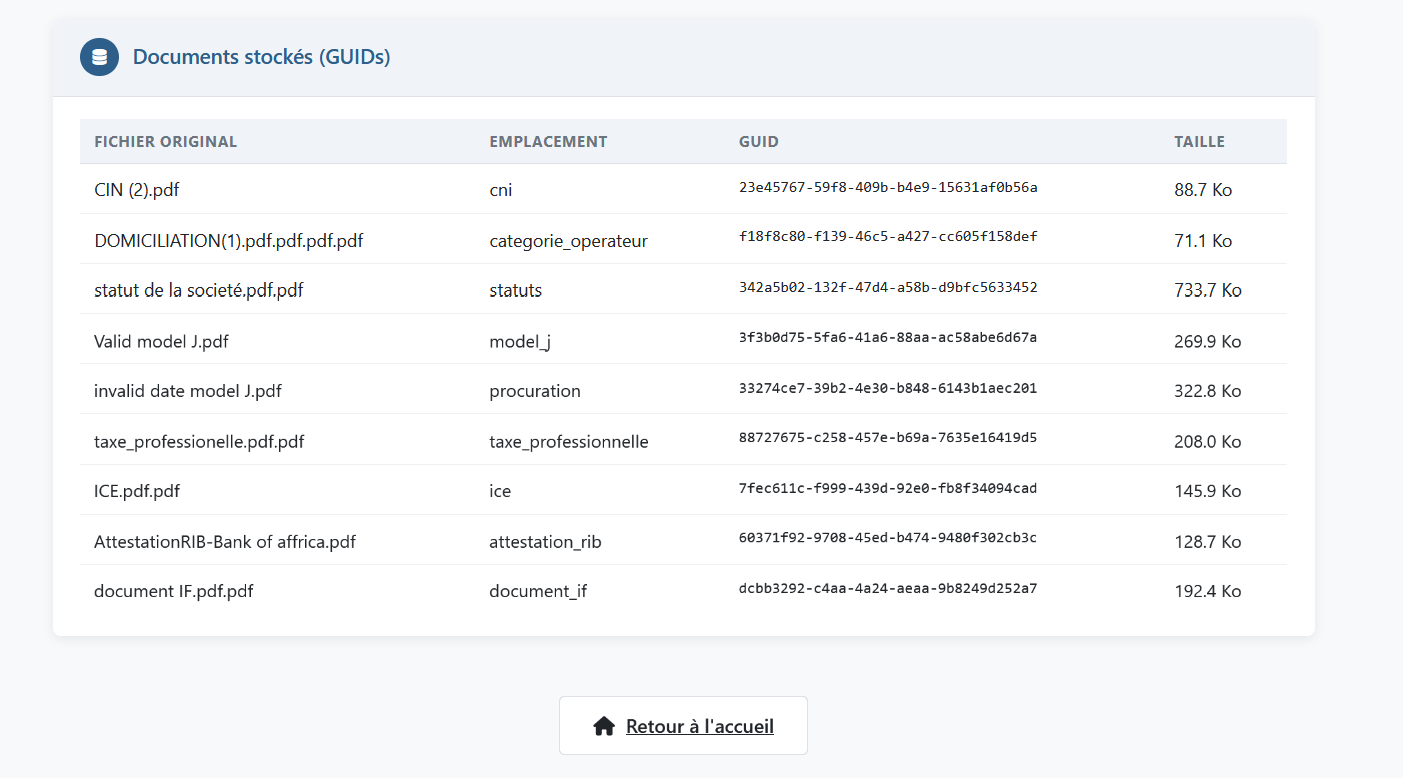
\includegraphics[width=0.85\textwidth]{Screenshots/documents_stockes_guids.png}
    \caption{Tableau des documents stock\'{e}s par le backend avec identifiants GUID, emplacement de classification et taille de fichier.}
    \label{fig:documents-stockes}
\end{figure}

Chaque fichier re\c{c}oit un GUID unique (ex. \texttt{23e45767-59f8-409b-b4e9-15631af0b56a}) garantissant l'unicit\'{e} et la tra\c{c}abilit\'{e} du stockage. La colonne \textit{Emplacement} confirme la classification automatique du document par le classifier (\texttt{cni}, \texttt{model\_j}, \texttt{attestation\_rib}, etc.).


\section{Frontend SPA}

Le frontend est une application mono-page de 586 lignes reproduisant fid\`{e}lement l'ergonomie du portail PortNet. Les principales fonctionnalit\'{e}s sont :

\begin{table}[H]
\centering
\small
\begin{tabularx}{\textwidth}{@{}>{\bfseries}p{3.5cm} Y@{}}
\toprule
\rowcolor{lightblue}
Fonctionnalit\'{e} & Description technique \\
\midrule
Authentification & \'{E}cran login/register avec captcha simul\'{e} et validation c\^{o}t\'{e} client \\
Wizard multi-\'{e}tapes & Navigation par onglets : Organisme $\to$ Formulaire $\to$ Documents $\to$ Validation \\
S\'{e}lection organisme & Choix PortNet+Douane ou Douane seule, conditionne les emplacements visibles \\
Formulaire dynamique & Champs conditionnels selon le type d'entit\'{e} (Personne Physique / Morale) \\
Upload Drag \& Drop & Zone de d\'{e}p\^{o}t HTML5 pour chaque emplacement de document \\
Validation visuelle & Badges color\'{e}s (vert/orange/rouge) avec messages d\'{e}taill\'{e}s par champ \\
Design System & Reproduction fid\`{e}le du portail PortNet (couleurs \texttt{\#16244a}, typographie Segoe UI) \\
\bottomrule
\end{tabularx}
\caption{Fonctionnalit\'{e}s du frontend SPA.}
\label{tab:frontend-features}
\end{table}

\subsection{\'{E}tape 4 : R\'{e}capitulatif des Informations de l'Op\'{e}rateur}

La figure~\ref{fig:formulaire-recap} pr\'{e}sente l'\'{e}tape~4 du wizard, o\`{u} les informations de l'op\'{e}rateur saisies aux \'{e}tapes pr\'{e}c\'{e}dentes sont r\'{e}capitulées avant le t\'{e}l\'{e}versement des documents. Ces donn\'{e}es (Raison Sociale, ICE, RC, IF, TP, Si\`{e}ge Social, Nom/Pr\'{e}nom/CIN du g\'{e}rant) serviront de r\'{e}f\'{e}rence pour la v\'{e}rification crois\'{e}e avec les valeurs extraites des documents.

\begin{figure}[H]
    \centering
    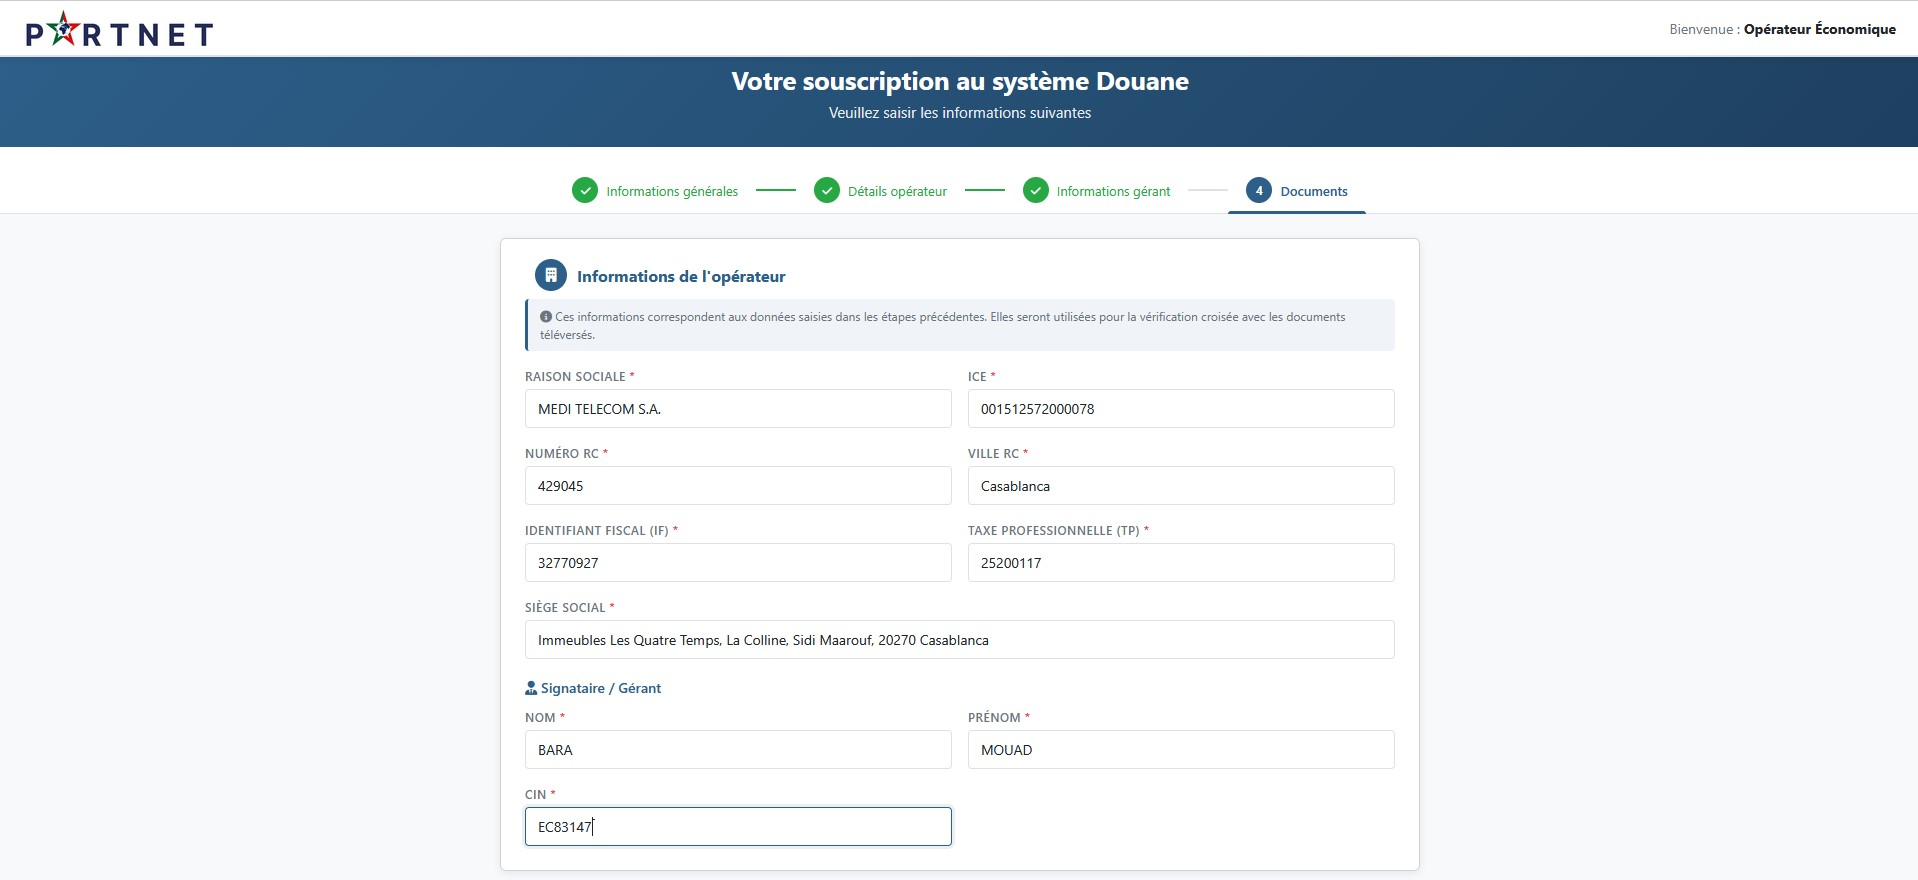
\includegraphics[width=0.82\textwidth]{Screenshots/formulaire_recap_operateur.jpg}
    \caption{\'{E}tape~4 du formulaire : r\'{e}capitulatif des informations de l'op\'{e}rateur avant le t\'{e}l\'{e}versement des documents.}
    \label{fig:formulaire-recap}
\end{figure}

\subsection{Zone d'Upload des Documents}

La figure~\ref{fig:upload-vide} pr\'{e}sente la zone de t\'{e}l\'{e}versement des documents dans son \'{e}tat initial, avant toute action de l'op\'{e}rateur. Chaque emplacement est \'{e}tiquet\'{e} selon le type de document attendu : \textit{Copie de la CIN}, \textit{Statut de la soci\'{e}t\'{e}}, \textit{Copie du mod\`{e}le J / Registre de commerce}, \textit{ICE}, \textit{Attestation de RIB}, \textit{Document IF}, \textit{Taxe Professionnelle}, \textit{Procuration} et \textit{Copie d'un document justifiant la cat\'{e}gorie de l'op\'{e}rateur}. L'astérisque (\texttt{*}) indique les champs obligatoires.

\begin{figure}[H]
    \centering
    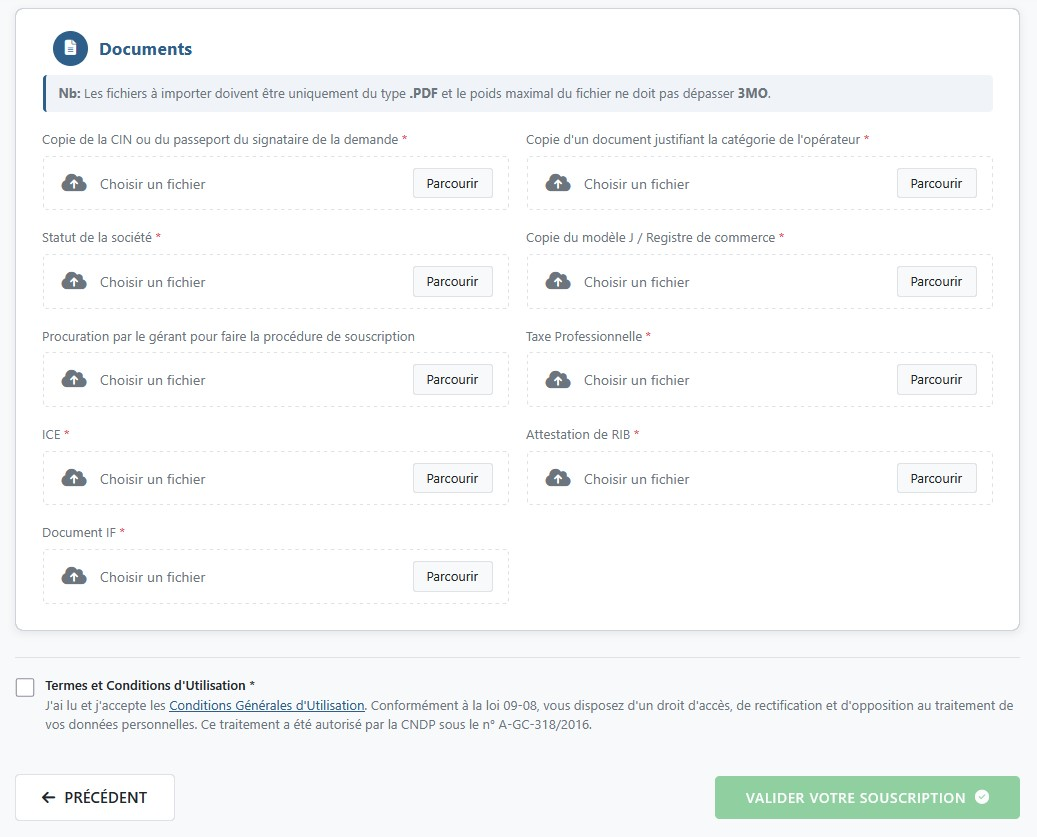
\includegraphics[width=0.82\textwidth]{Screenshots/upload_documents_vide.jpg}
    \caption{Zone d'upload des documents dans son \'{e}tat initial (aucun fichier d\'{e}pos\'{e}).}
    \label{fig:upload-vide}
\end{figure}

\subsection{Classification et Validation en Temps R\'{e}el}

D\`{e}s qu'un fichier PDF est d\'{e}pos\'{e} dans un emplacement, le syst\`{e}me ex\'{e}cute le pipeline de classification en temps r\'{e}el. La figure~\ref{fig:upload-valides} montre le r\'{e}sultat apr\`{e}s le t\'{e}l\'{e}versement de documents valides : chaque emplacement affiche un badge vert \guillemotleft~Document conforme~\guillemotright{} suivi du type d\'{e}tect\'{e} (par exemple, \textit{Carte Nationale d'Identit\'{e} / Passeport}, \textit{Mod\`{e}le J / Registre de commerce}).

Le champ \textit{Procuration} affiche un badge bleu \guillemotleft~Ce document sera v\'{e}rifi\'{e} manuellement par un agent~\guillemotright{}, car la procuration ne fait pas l'objet d'une v\'{e}rification automatis\'{e}e.

\begin{figure}[H]
    \centering
    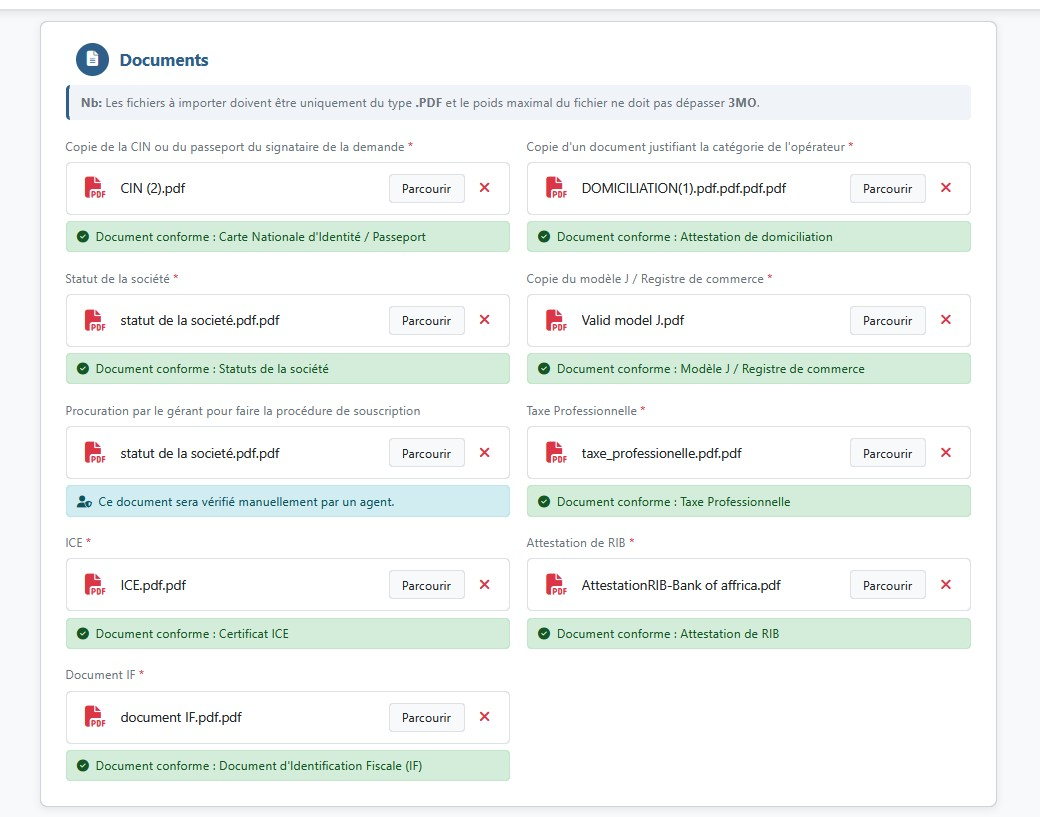
\includegraphics[width=0.82\textwidth]{Screenshots/upload_documents_valides.jpg}
    \caption{Documents t\'{e}l\'{e}vers\'{e}s avec succ\`{e}s : chaque emplacement affiche un badge vert \guillemotleft~Document conforme~\guillemotright.}
    \label{fig:upload-valides}
\end{figure}

La figure~\ref{fig:upload-bouton} montre le bas de la page avec la case \guillemotleft~Termes et Conditions d'Utilisation~\guillemotright{} coch\'{e}e et le bouton \guillemotleft~Valider votre souscription~\guillemotright{} activ\'{e}, permettant \`{a} l'op\'{e}rateur de soumettre son dossier complet au pipeline de v\'{e}rification.

\begin{figure}[H]
    \centering
    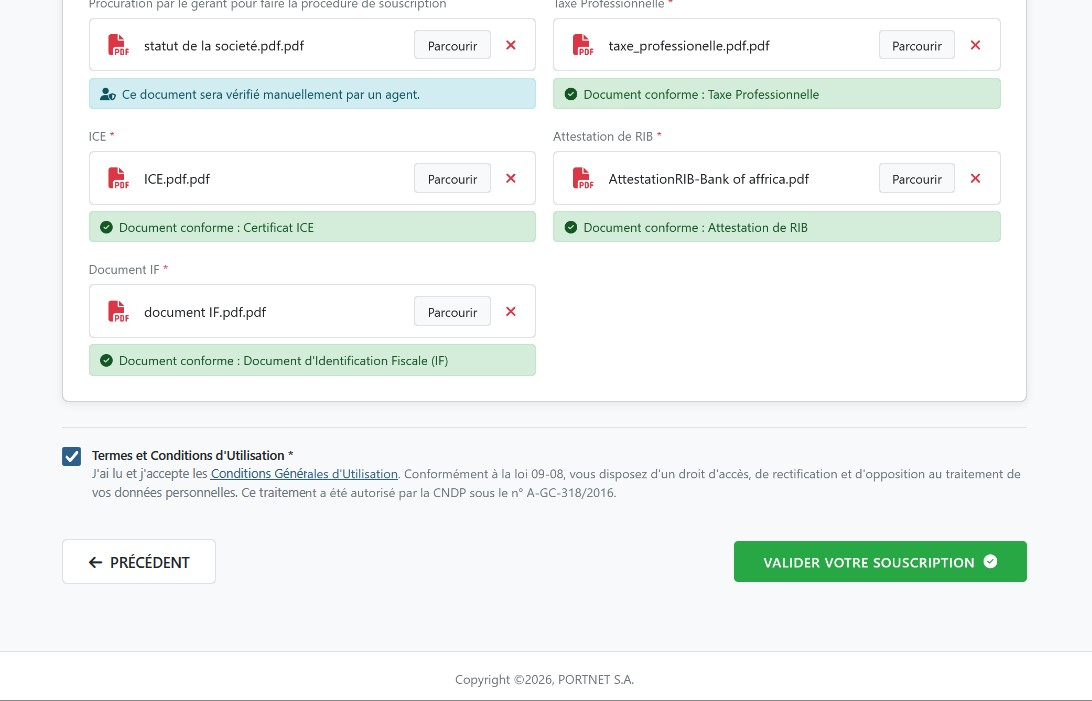
\includegraphics[width=0.82\textwidth]{Screenshots/upload_documents_bouton_valider.jpg}
    \caption{Bas de page : case \guillemotleft~Termes et Conditions~\guillemotright{} coch\'{e}e et bouton de soumission activ\'{e}.}
    \label{fig:upload-bouton}
\end{figure}

\section{Correspondance Floue (Fuzzy Matching)}

\begin{lstlisting}[language=Python, caption={Module de correspondance floue (fuzzy\_match.py).}, label={lst:fuzzy-match}]
from rapidfuzz import fuzz
from souscription.config.settings import (
    FUZZY_NAME_THRESHOLD,   # 85.0
    FUZZY_ADDRESS_THRESHOLD # 75.0
)

def match_names(name1, name2, threshold=FUZZY_NAME_THRESHOLD):
    """Compare company names using token_set_ratio."""
    score = fuzz.token_set_ratio(
        normalize_text(name1),
        normalize_text(name2)
    )
    return score >= threshold, score

def match_addresses(addr1, addr2, threshold=FUZZY_ADDRESS_THRESHOLD):
    """Compare addresses using token_set_ratio."""
    score = fuzz.token_set_ratio(
        normalize_text(addr1),
        normalize_text(addr2)
    )
    return score >= threshold, score
\end{lstlisting}

\section*{Conclusion du Chapitre}

Ce chapitre a pr\'{e}sent\'{e} la r\'{e}alisation technique compl\`{e}te du syst\`{e}me, depuis le pipeline d'ingestion \`{a} trois niveaux jusqu'au frontend SPA. Chaque composant a \'{e}t\'{e} illustr\'{e} par des listings de code source extraits directement du projet, accompagn\'{e}s de sch\'{e}mas architecturaux. Le Chapitre~5 pr\'{e}sentera les r\'{e}sultats de la campagne de tests et l'\'{e}valuation des performances du syst\`{e}me.
